\subsection{OS Replacement}
%\subsubsection{OS Replacement}
We run our experiments on a server machine equipped with two 6-core Intel Xeon CPUs of 2.1 GHz and 128 GB memory. We use KVM/QEMU to run source and destination VMs on the same server host. Both VMs are configured with 4 VCPUs and 4 GB memory. \arch's OS replacement is implemented with CRIU version 3.5. 
%Table \ref{tab:experiment1}. shows the configuration of the hyperplexor and the VMs.

\begin{figure}
	\centering
	\subfloat[Replacement time]{
		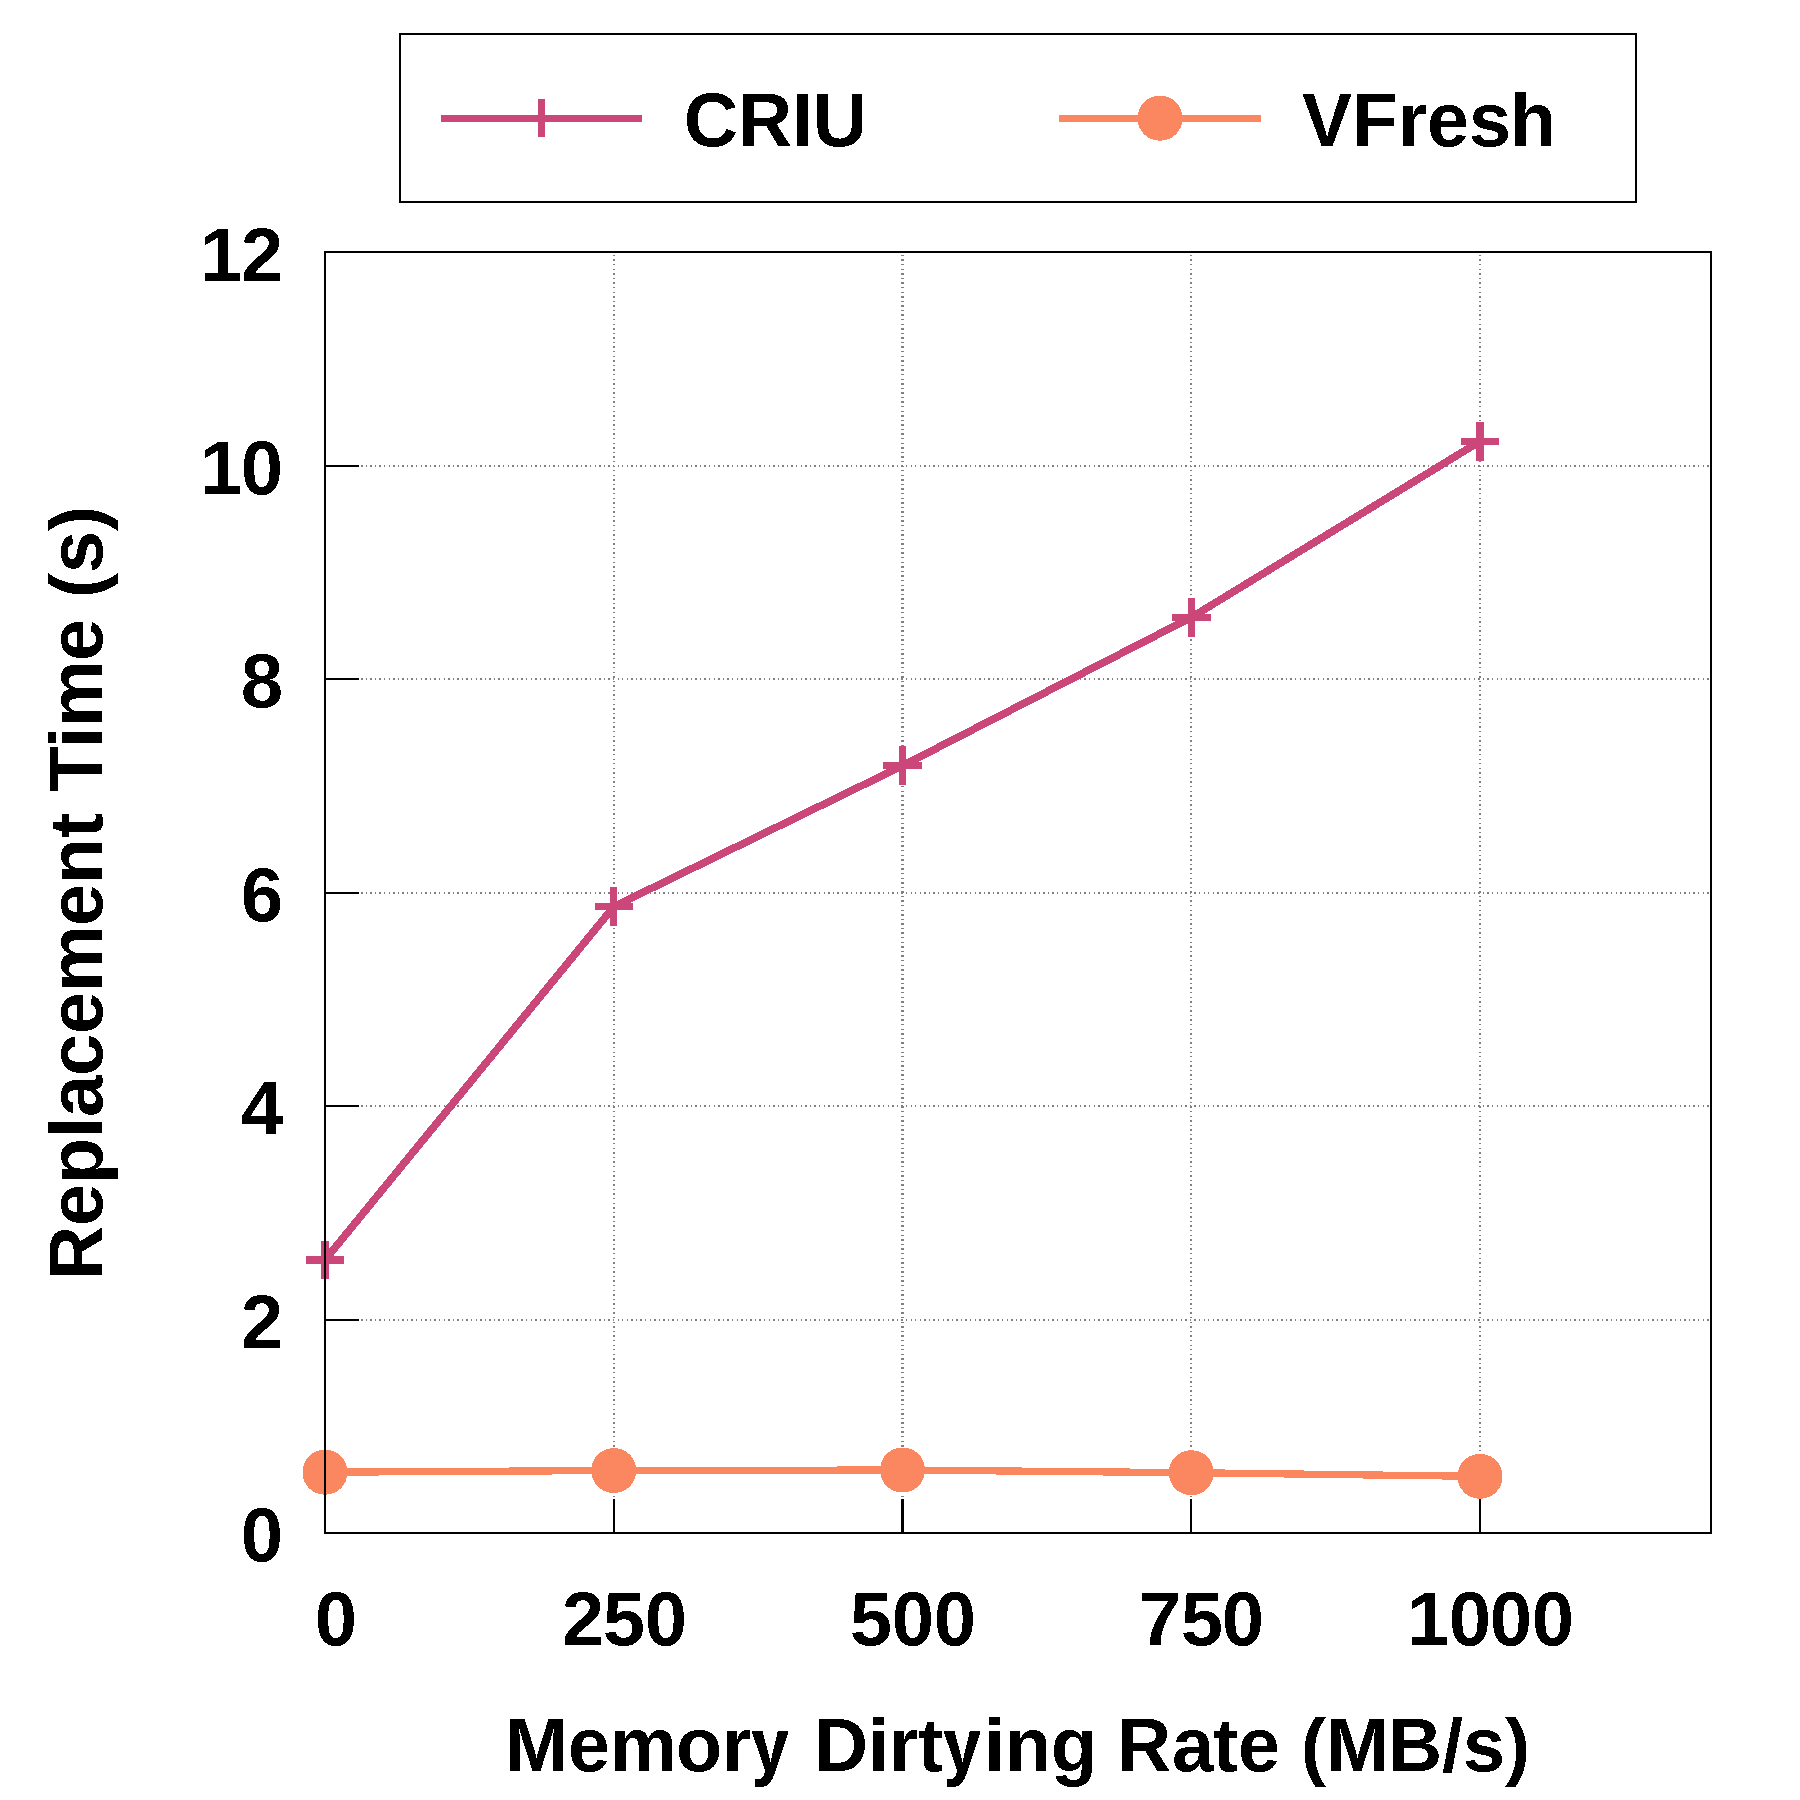
\includegraphics[width=.235\textwidth]{figures/memory_dirty_rate_process_migration_tmt.pdf}}
	\subfloat[Frozen time]{
		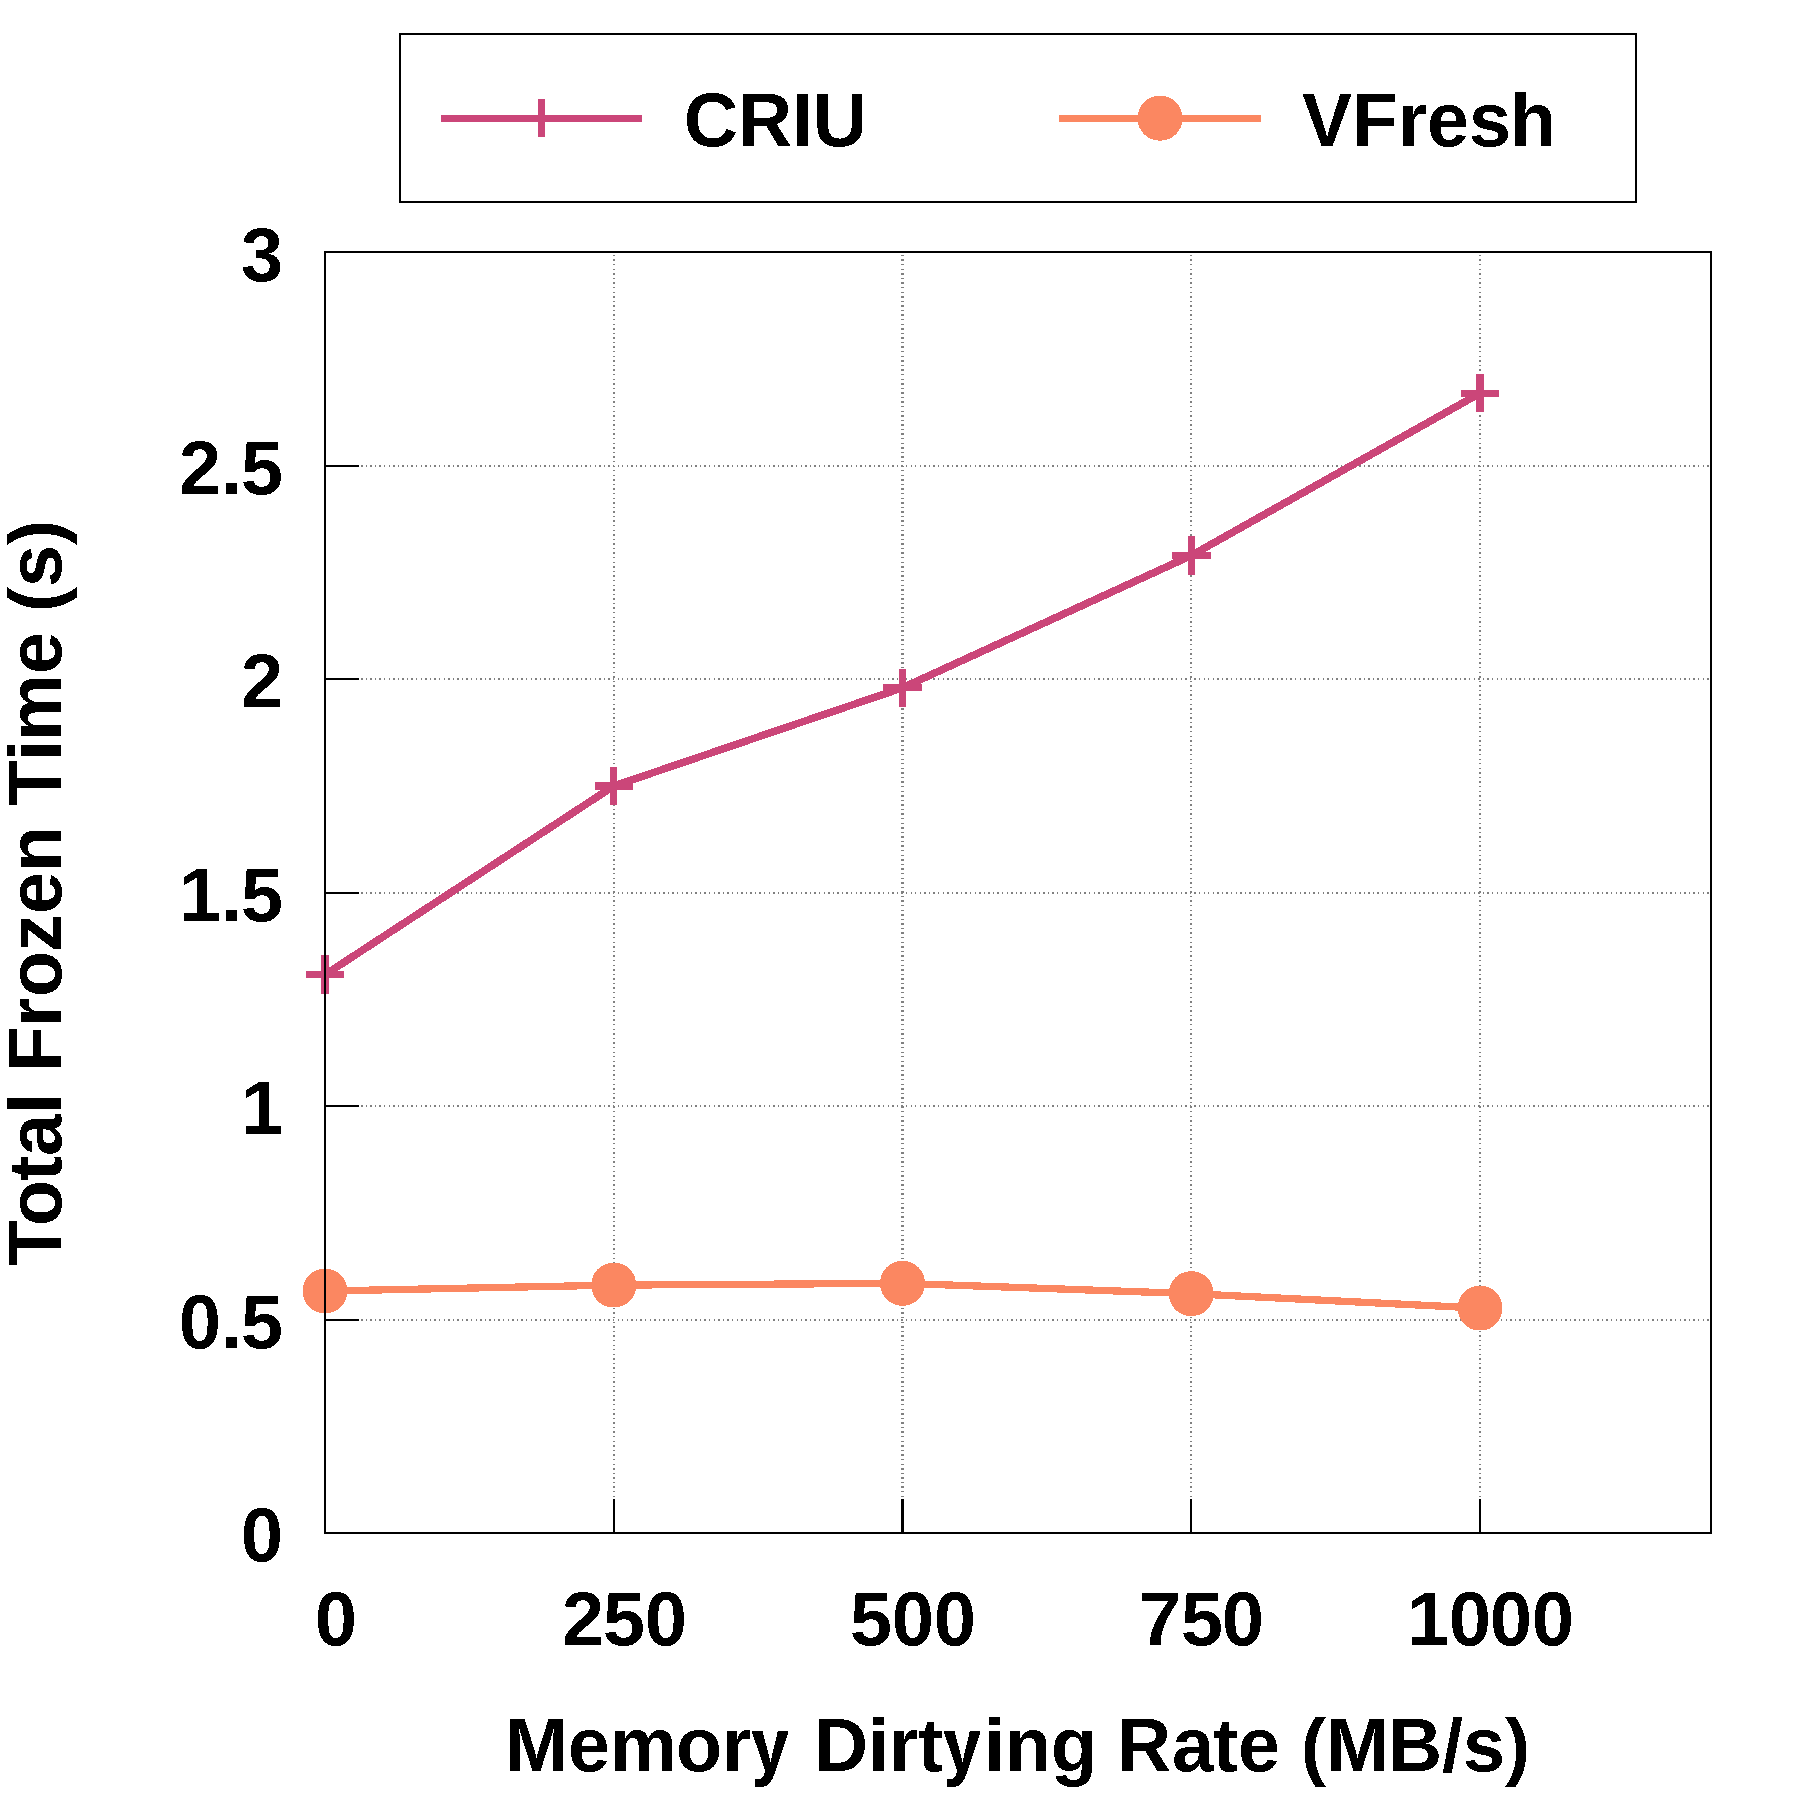
\includegraphics[width=.235\textwidth]{figures/memory_dirty_rate_process_migration_tft.pdf}}
	\caption{Effect of memory intensive workload on OS replacement.}
	\label{fig:variation23}
    \vspace{0.2in}
\end{figure}

\begin{figure*}
	\centering
    \subfloat[Sysbench]{
		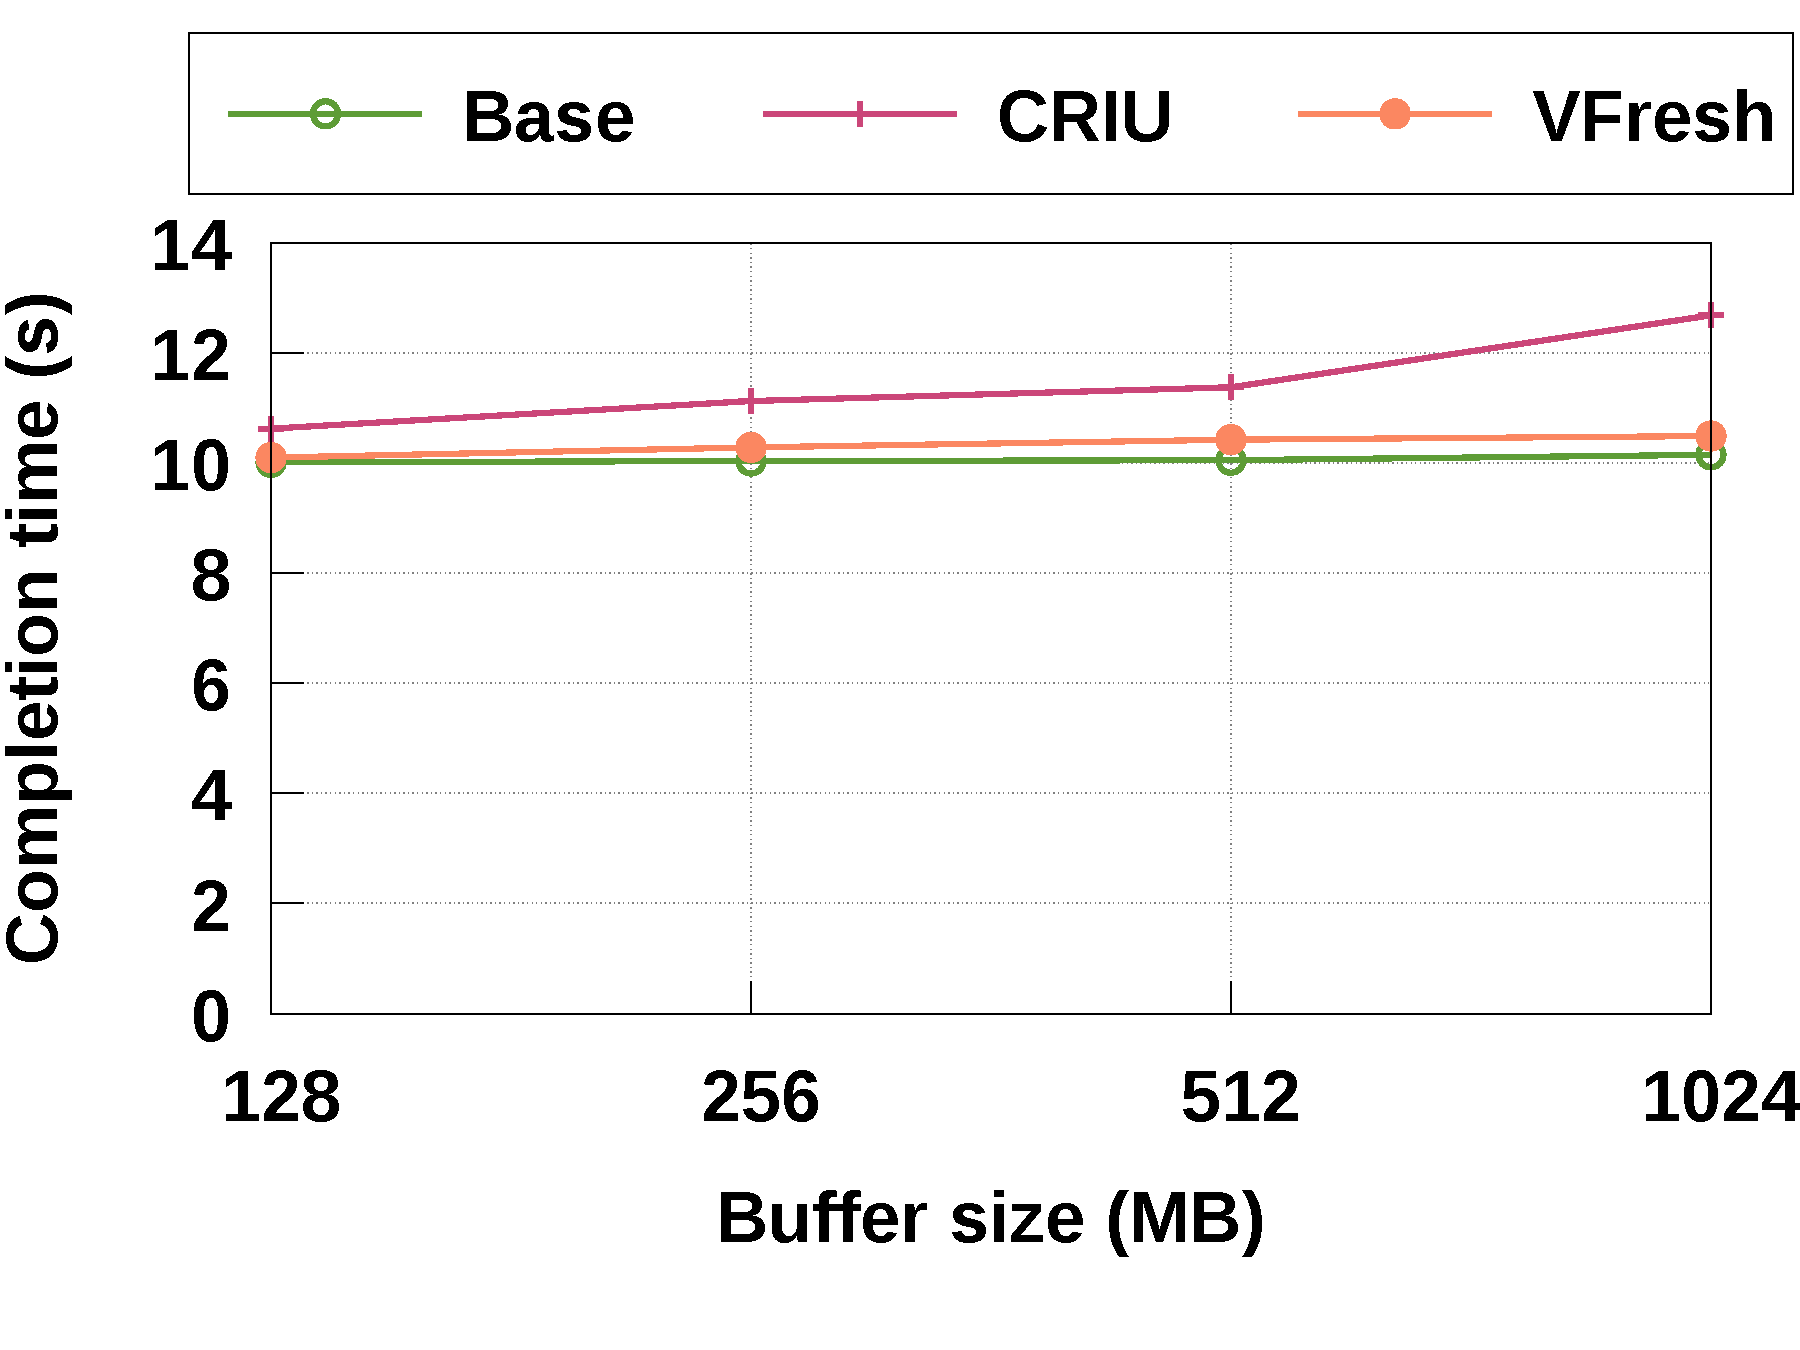
\includegraphics[width=.24\textwidth]{figures/sysbench_performance.pdf}}
		%\hspace{0.1in}
	\subfloat[Parsec]{
		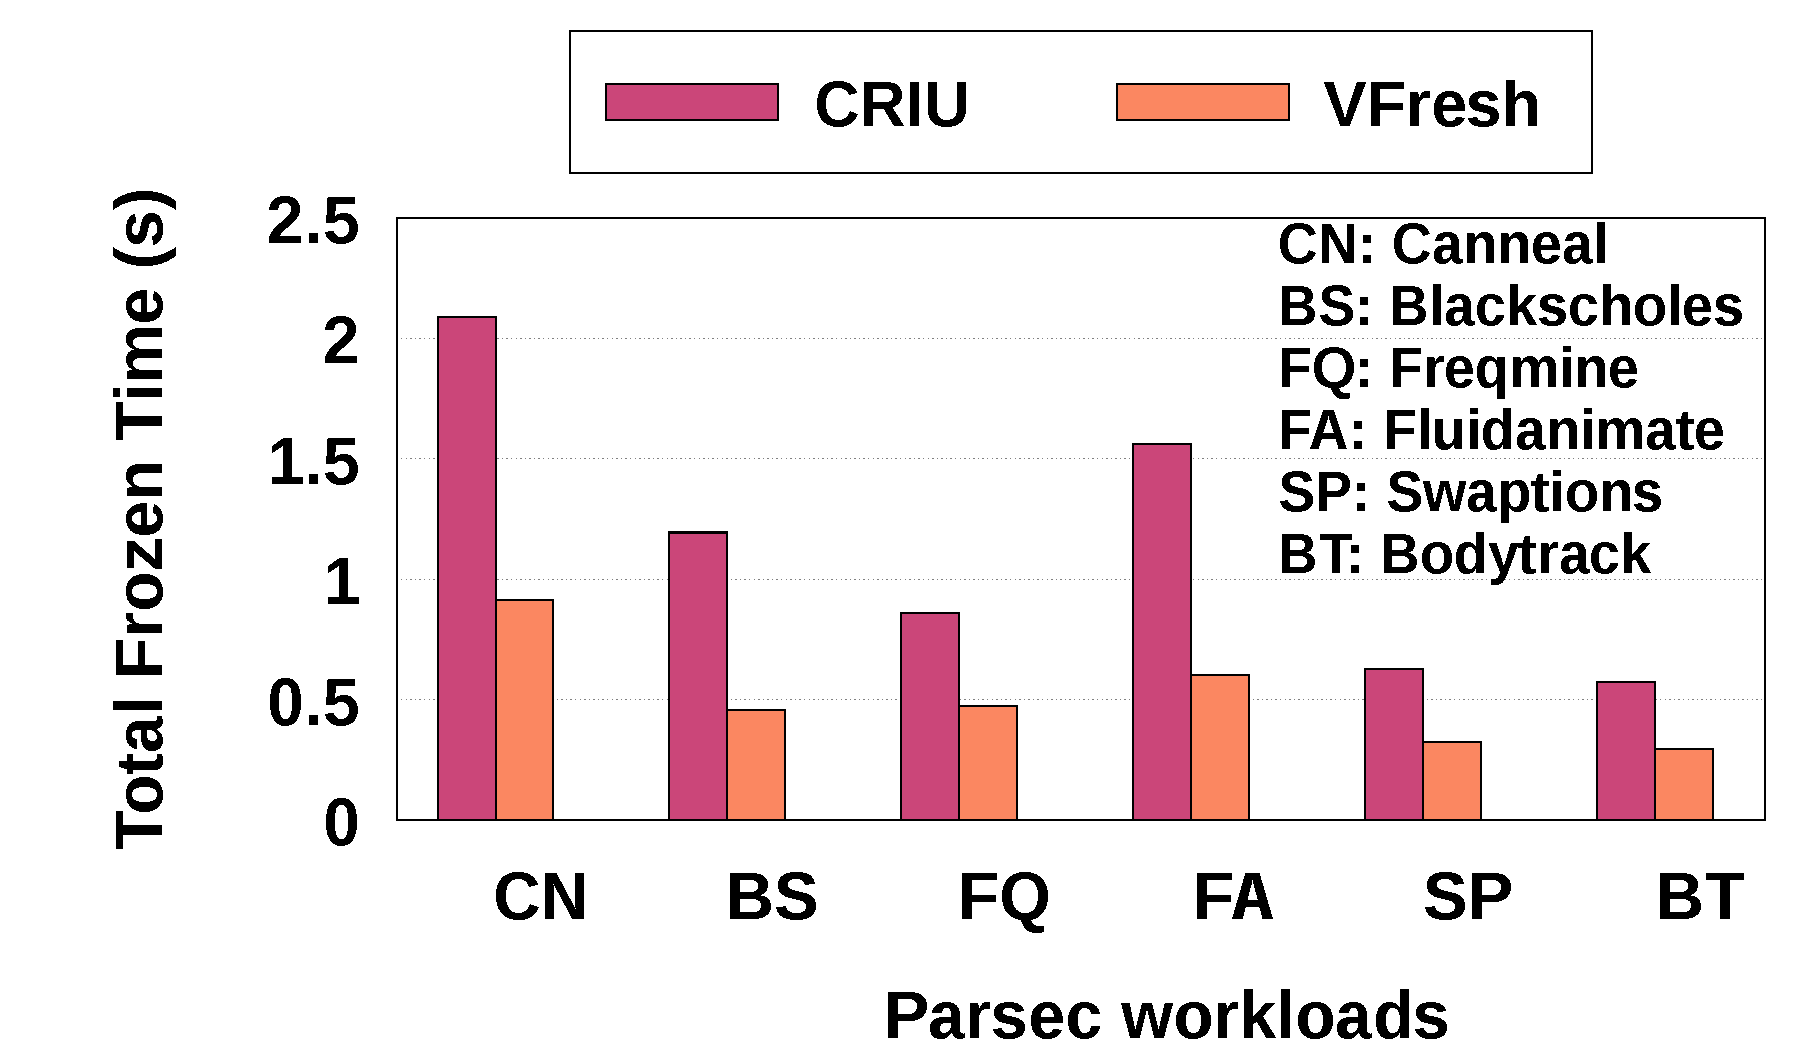
\includegraphics[width=.328\textwidth]{figures/parsec.pdf}}
		\hspace{-0.1in}
    \subfloat[Quicksort]{
		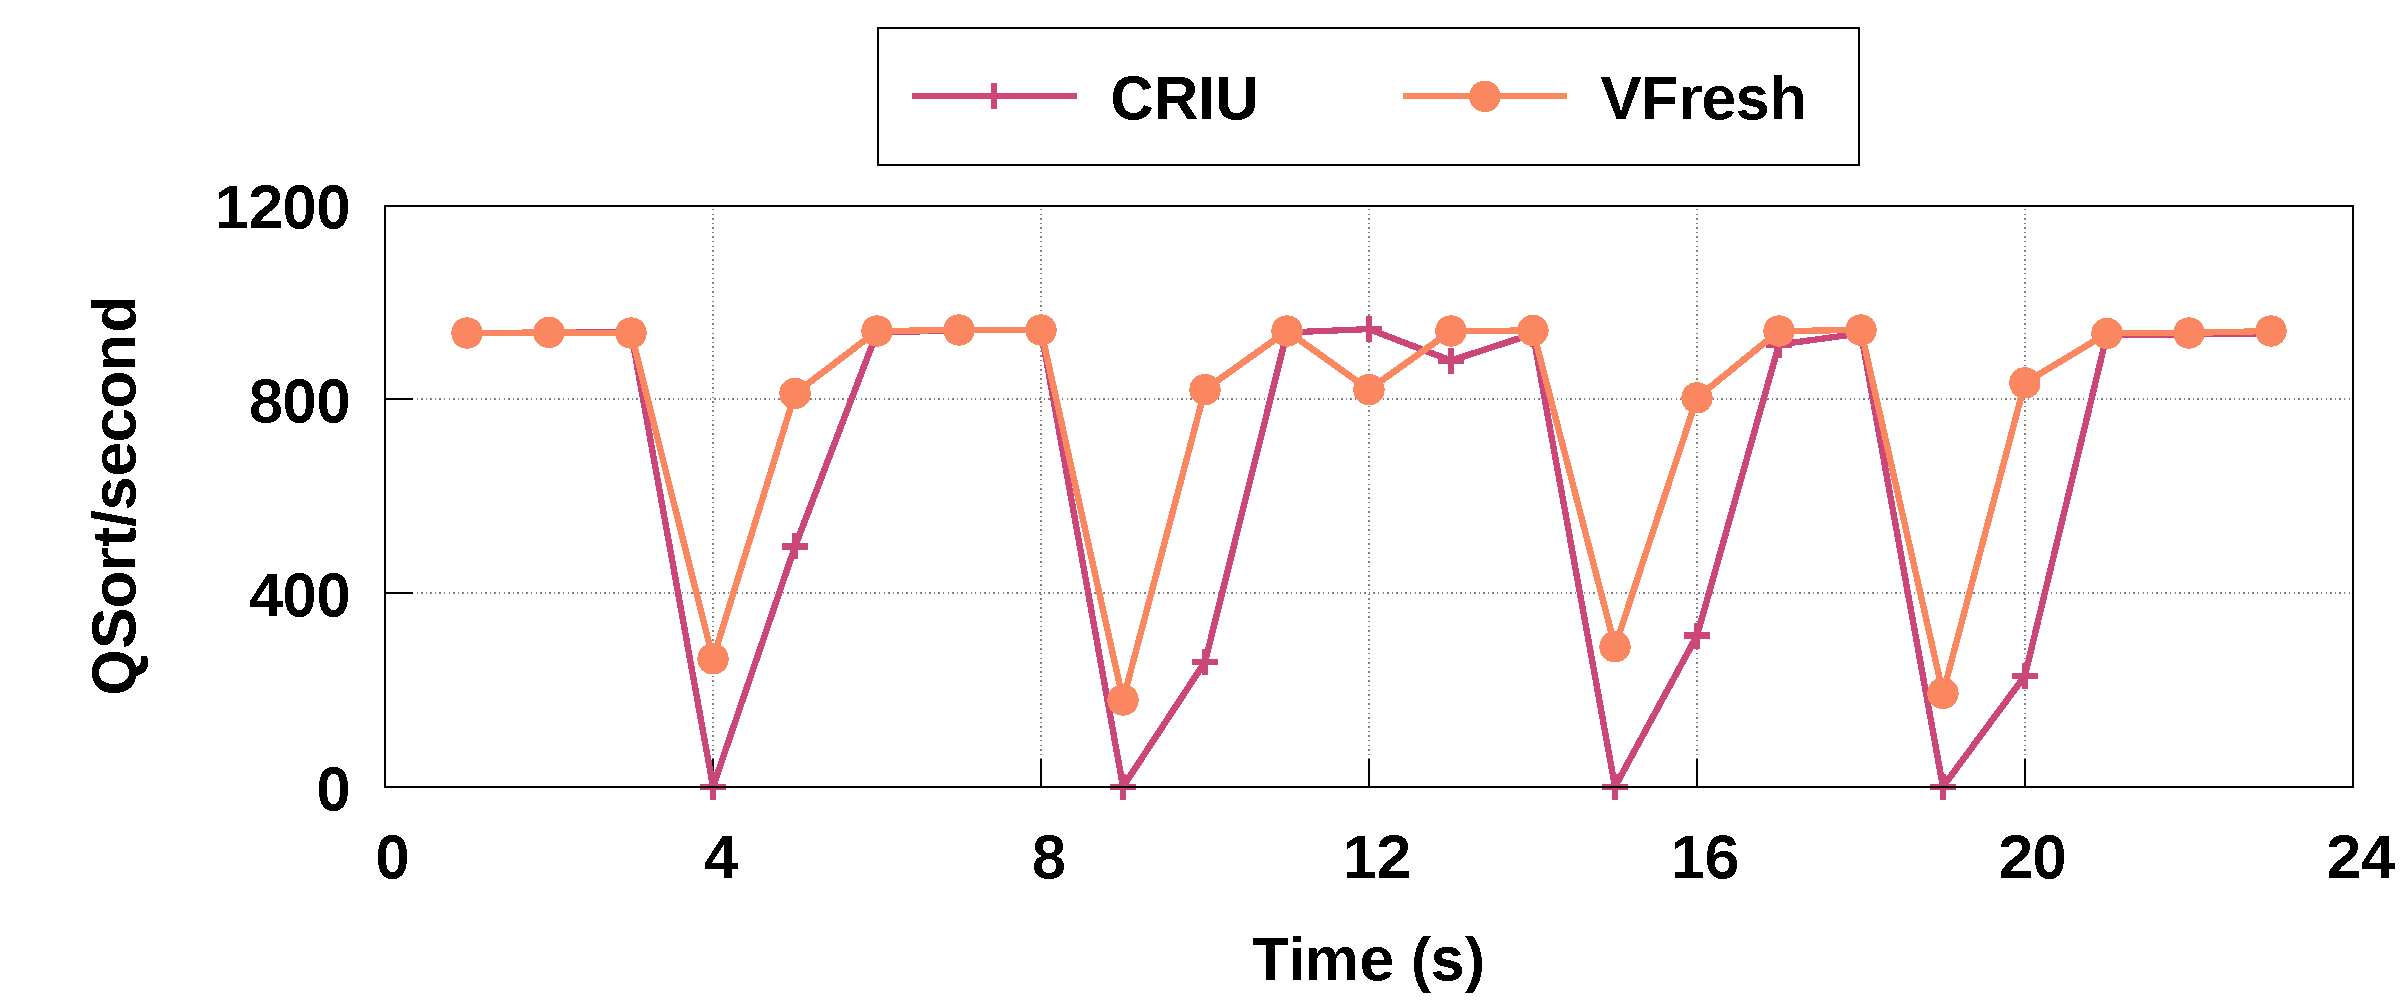
\includegraphics[width=.42\textwidth]{figures/quicksort_performance.pdf}}
	%\hspace{0.1in}
		%\vspace{-0.1in}
	\caption{Comparison of application performance for OS replacement.}
	%\vspace{-0.1in}
	\label{fig:impl1}
\end{figure*}
%\begin{table}
%	\begin{tabular}{|c|c|c|}
%		\hline
%		 Hyperplexor & VM (stale OS) & VM (replacement OS) \\
%		\hline
%		128GB, 12 CPUs    & 4GB, 4 VCPUs    & 4GB, 4 VCPUs \\
%		\hline
%	\end{tabular}
%	
%	\caption{Setup for OS replacement experiments}
%	\label{tab:experiment1}
%\end{table}

\subsubsection{Replacement Time}
We measure the OS replacement time under \arch and compare it with the pre-copy live migration approach (implemented based on PHaul \cite{phaul}). We run a container with one process which allocates 1 GB memory and then continuously performs write operations to the memory pages at varying rates from 0 MB/second (i.e., no dirty pages) to 1 GB/second (i.e., all pages are dirtied each second). We compare the total OS replacement time and the container downtime (i.e., frozen time).

\fref{fig:variation23} shows that, with the pre-copy live migration approach the total OS replacement time and the frozen time increase as the memory dirty rate increases. For example, the replacement time is around 2.5 seconds when the dirty rate is 0, and increases to 10 seconds when the dirty rate is 1 GB/second. The frozen time is around 1.7 seconds when the dirty rate is 0, and increases to 2.7 seconds when the dirty rate is 1 GB/second. In contrast, with \arch, the total replacement time and frozen time remain constant, around 0.5 seconds (i.e., the total replacement time equals to the frozen time in \arch). Because \arch transfers the memory ownership instead of copying memory pages, it leads to much shorter OS replacement time and frozen time compared with the pre-copy based approach. 

We notice that the OS replacement time (0.5 seconds with 1 GB memory) is higher than the hypervisor replacement time (e.g., 10 ms). The main reason is that, \arch's OS replacement builds on a popular user space checkpointing/restoration tool (i.e., CRIU), which incurs high overhead in collecting state of processes during which processes are paused. A low-overhead, kernel-level solution is a subject of our ongoing investigations.

%the effect of container's memory usage on the OS replacement time. We start a container with memory intensive processes which allocate 1 GB memory and perform a continuous write operation on it at a varying rate ranging from 0MB/second to 1GB/second. We compare the OS replacement time of VFresh with CRIU. To complete the OS replacement, CRIU takes multiple iterations to send all the memory state. With increase in memory writing rate, memory getting dirtied during each iteration increases. Hence, the replacement time and the downtime increases as well. Additionally, if the iterations are not stopped manually, then the replacement operation will never complete, reason being the size of the dirtied memory during the iterations is not converging. However, OS replacement and downtime using \arch stay not only very small compared to CRIU, but also constant with variation in memory writing rate. Since VFresh is not iterative and the total memory usage is constant, so the replacement time doesn't get affected by the change in memory writing rate. 



\subsubsection{Performance Impact}
\label{sec:workload}

We use the following three macro-benchmarks to show performance impact during OS replacement.

\para{Sysbench} \cite{sysbench} provides multi-threaded memory testing by reading from or writing to preallocated memory. In our experiments, we preallocate a buffer with varying sizes from 128 MB to 1 GB, and perform write operations to this buffer repetitively till its completion --- a total size of memory has been written (i.e., 1,000 GB in our experiments). We compare three cases: (a) the baseline without OS replacement; (b) pre-copy based approach using CRIU; and (c) \arch. In cases (b) and (c), we conduct one OS replacement during each run.

%We use this benchmark to show the total completion time of a write-intensive experiment.

In Figure \ref{fig:impl1}a, the completion time under \arch is almost the same as the baseline (without OS replacement). On the contrary, the pre-copy based approach takes longer time to complete for each run. Further, the completion time increases as the buffer size increases --- the large the buffer size, the more memory pages needed to be copied for the pre-copy based approach. 
%the completion time
%we compare the sysbench completion time while changing the buffer size from 128MB to 1024MB. The baseline data represents the completion time of sysbench a VM. To compare with this baseline data, we migrate a running sysbench application and observe its completion time after migration. Performance of sysbench with migration using \arch is almost similar to baseline. However, sysbench takes much longer time to complete when migrated using CRIU. Furthermore, its completion time using CRIU increases more rapidly with the increment in buffer size. In \arch the change in completion time is not significant.

\para{Parsec} \cite{parsec} benchmark mimics large-scale commercial applications. We run a variety of sub workloads of parsec benchmark, during which we perform OS replacement. As each workload takes a long time to complete, we compare the total frozen time during the OS replacement between \arch and the pre-copy based approach.


\fref{fig:impl1}b shows that the total frozen time for workloads with higher memory usage is longer than workloads with lower memory usage. For example, canneal and fluidanimate have very high memory usage, whereas swaptions and bodytrack use only a small amount of memory. Hence, canneal and fluidanimate have longer frozen time during the OS replacement than swaptions and bodytrack. Yet, the total frozen time of all the workloads with \arch is almost half the size of that with the pre-copy based approach.
%Figure \ref{fig:impl1} (b) compares the total frozen time of different workloads of parsec benchmark while being migrated using \arch and CRIU. We have used workloads with varying memory usage. We observe that the total frozen time for workloads with high memory usage is higher compared to workloads with lower memory usage. For example, canneal and fluidanimate workload have very high memory usage whereas swaptions and bodytrack use only a small amount of memory. Hence, canneal and fluidanimate workloads are frozen longer during migration compared to swaptions and bodytrack. However, the total frozen time of the workloads using \arch is almost half compared to CRIU.

\para{Quicksort} is used again to show the number of quicksort operations per second, when we conduct multiple OS replacements. Figure \ref{fig:impl1}c shows that, the number of quicksort operations per second during OS replacement reduces to zero for a short period of time with the pre-copy based approach. In contrast, with \arch, we observe at least 200$\sim$400 quicksort operations per second during the OS replacement. This is because, the frozen time with \arch is much smaller than that with the pre-copy based approach.

%\begin{figure*}
%	\centering
%	
%	\subfloat[Total Migration Time]{
%		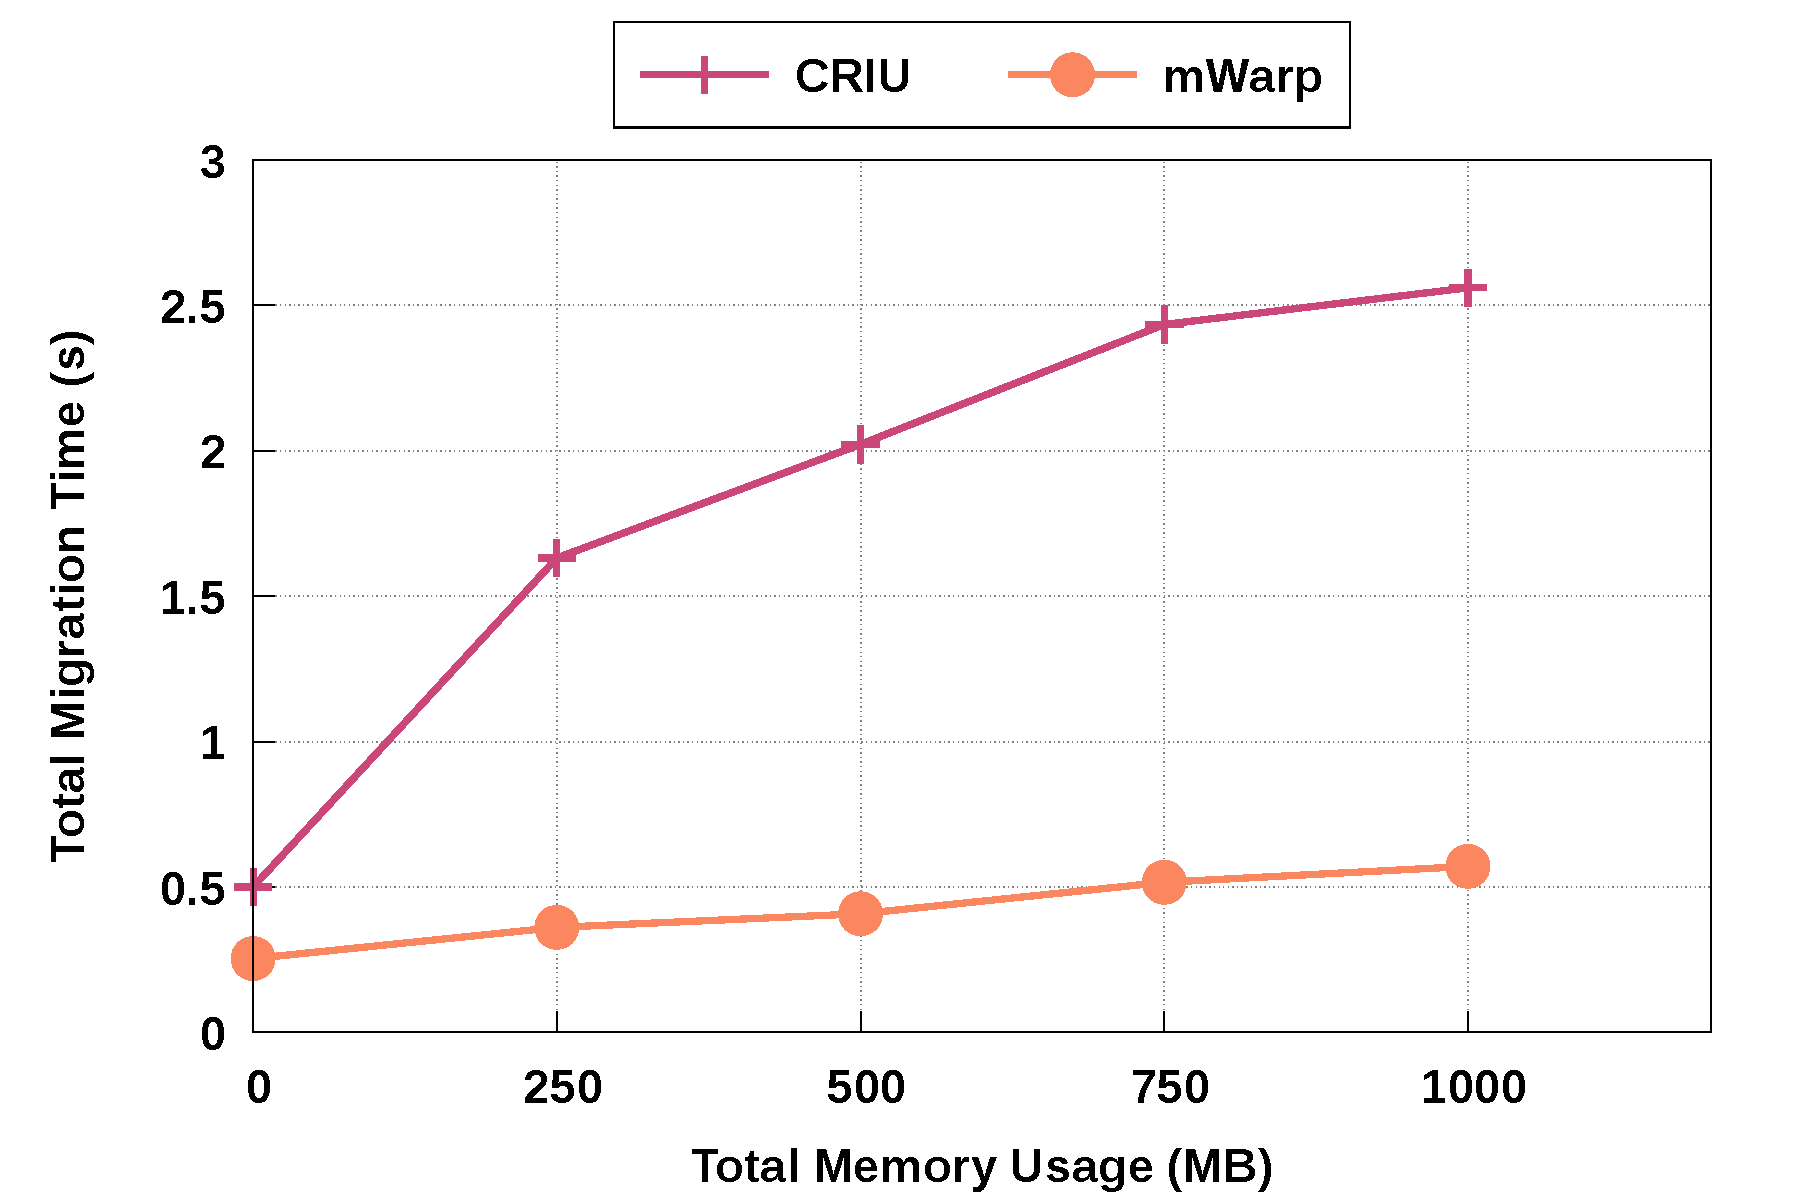
\includegraphics[width=.5\textwidth]{figures/memory_usage_process_migration_tmt.pdf}}
%	\subfloat[Total Frozen Time]{
%		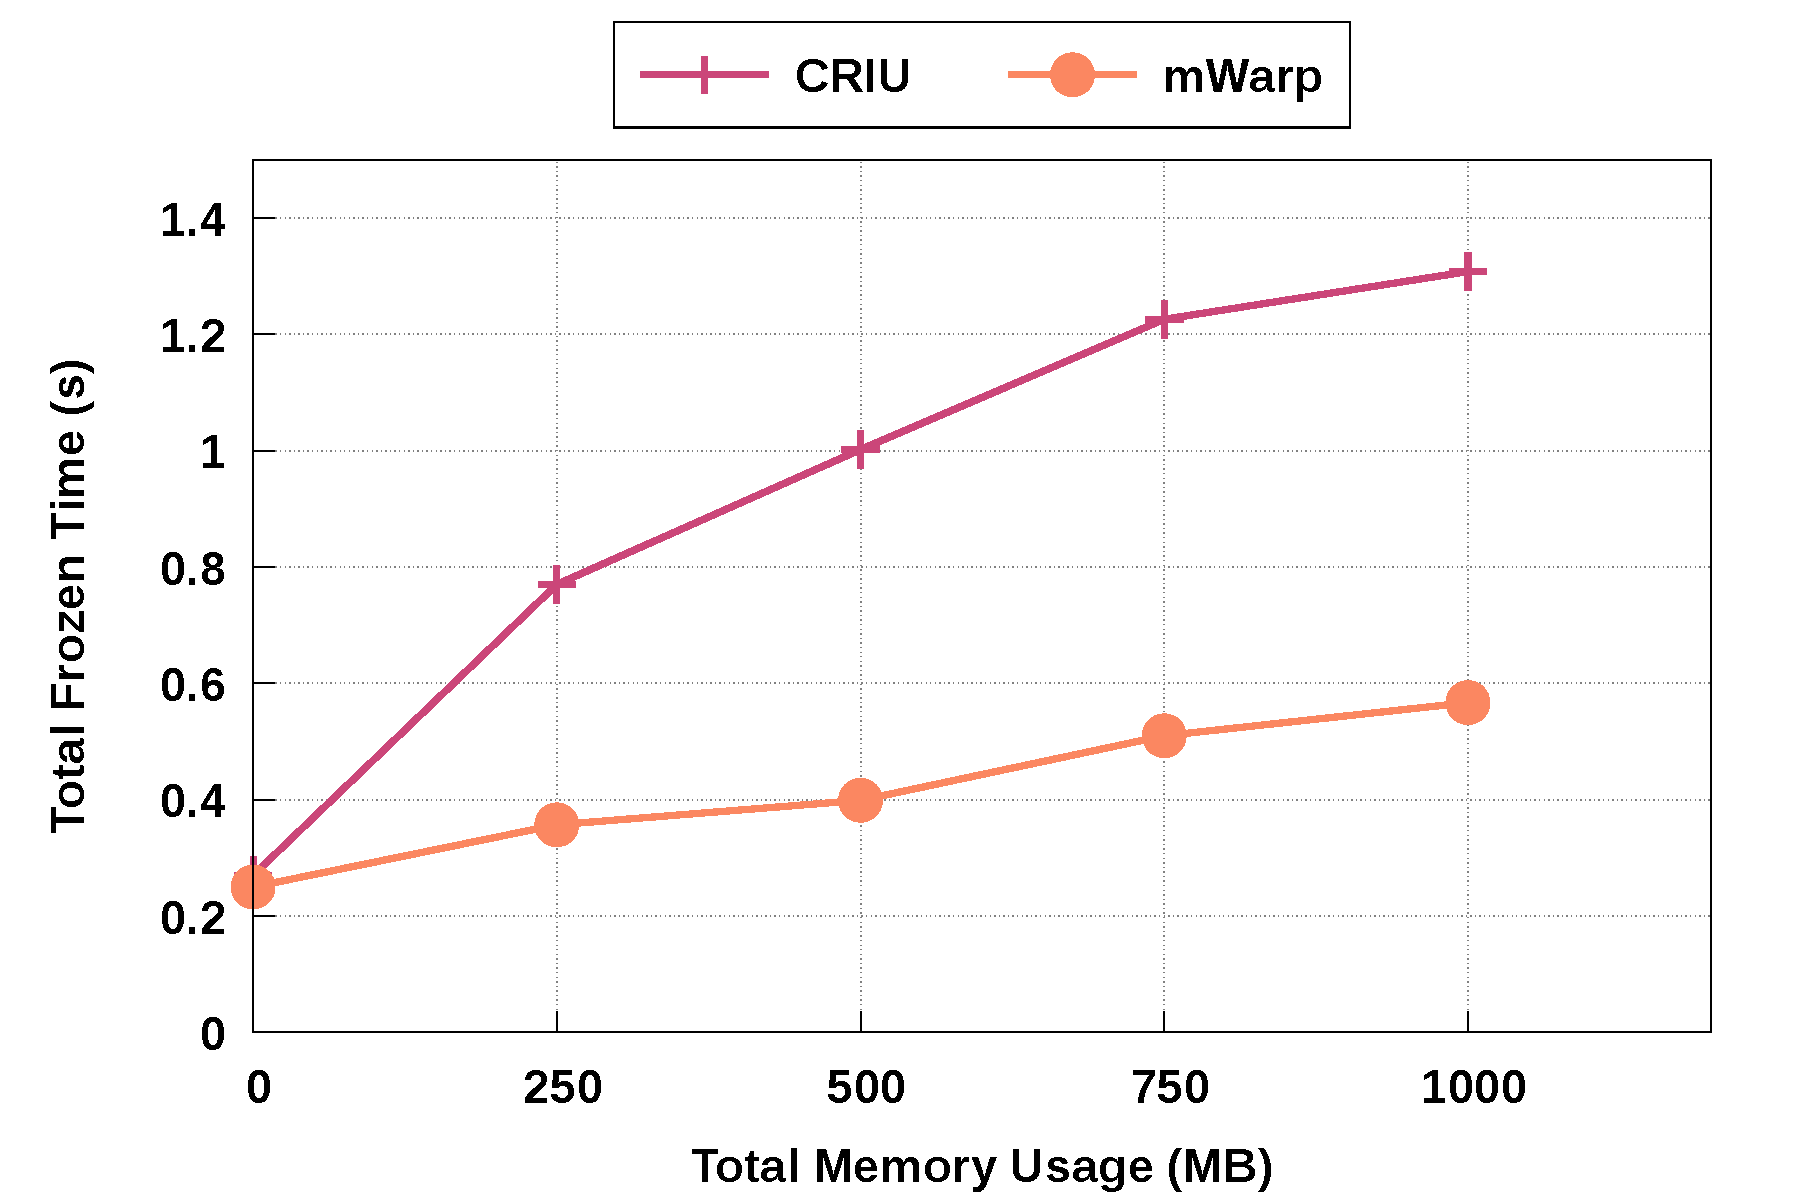
\includegraphics[width=.5\textwidth]{figures/memory_usage_process_migration_tft.pdf}}
%	\caption{Memory Size Variations}
%	\label{fig:variation1}
%\end{figure*}
%\begin{figure*}
%	\centering
	
%	\subfloat[Total Migration Time]{
%		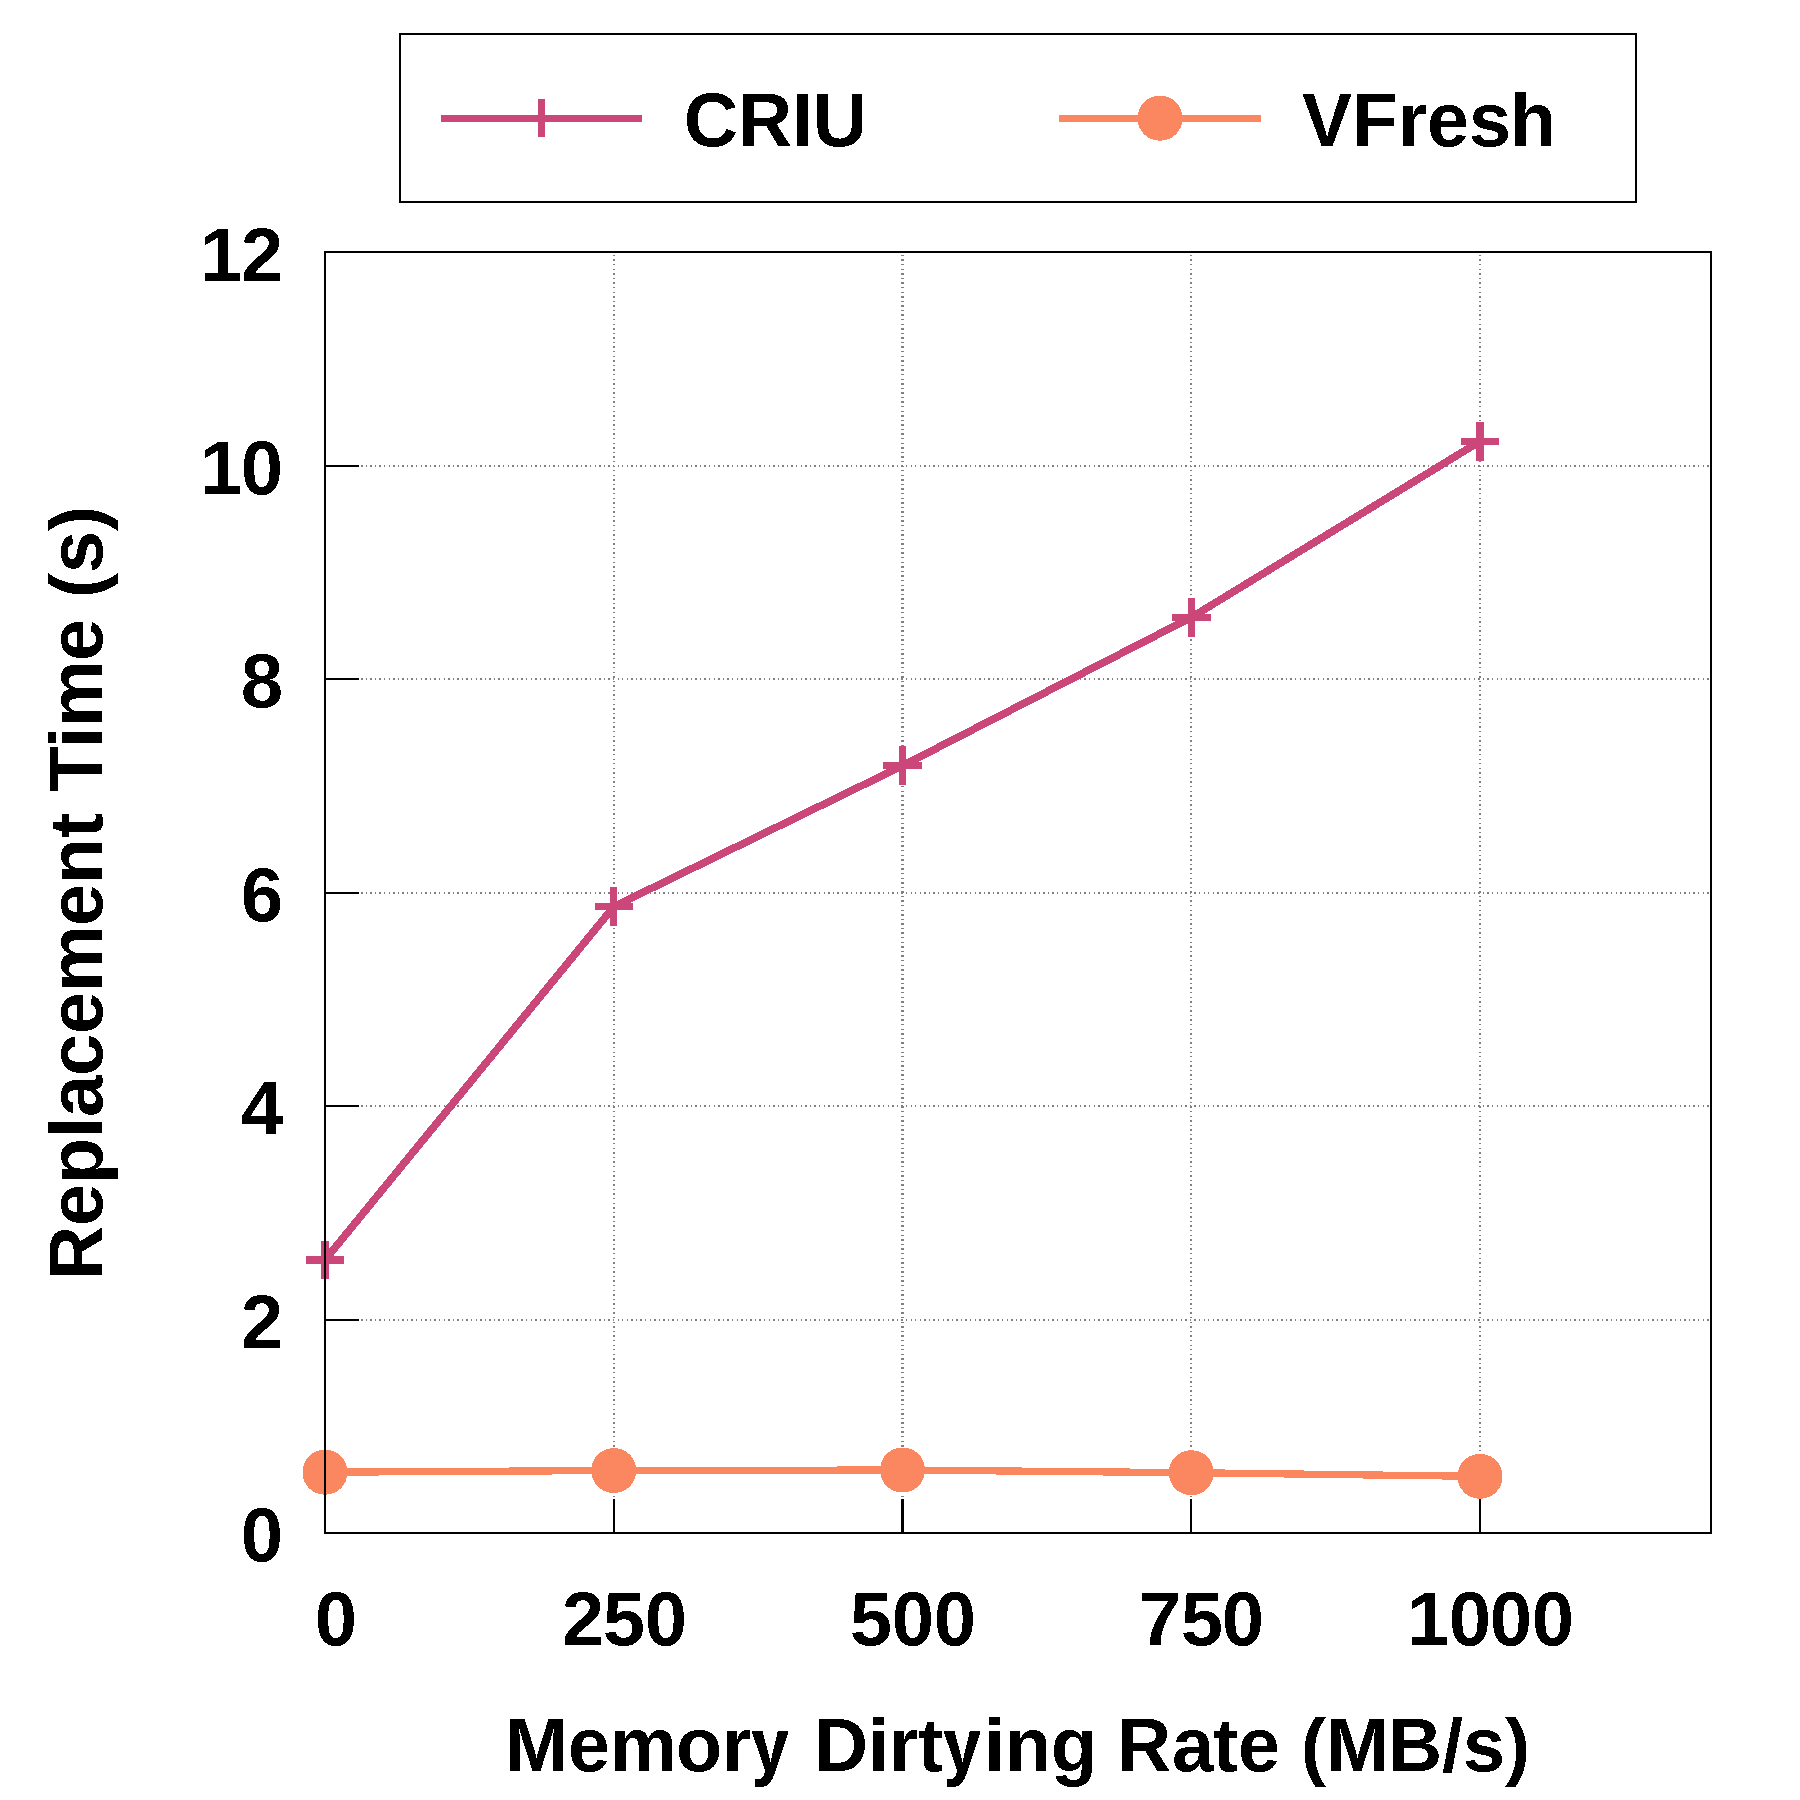
\includegraphics[width=.5\textwidth]{figures/memory_dirty_rate_process_migration_tmt.pdf}}
%	\subfloat[Total Frozen Time]{
%		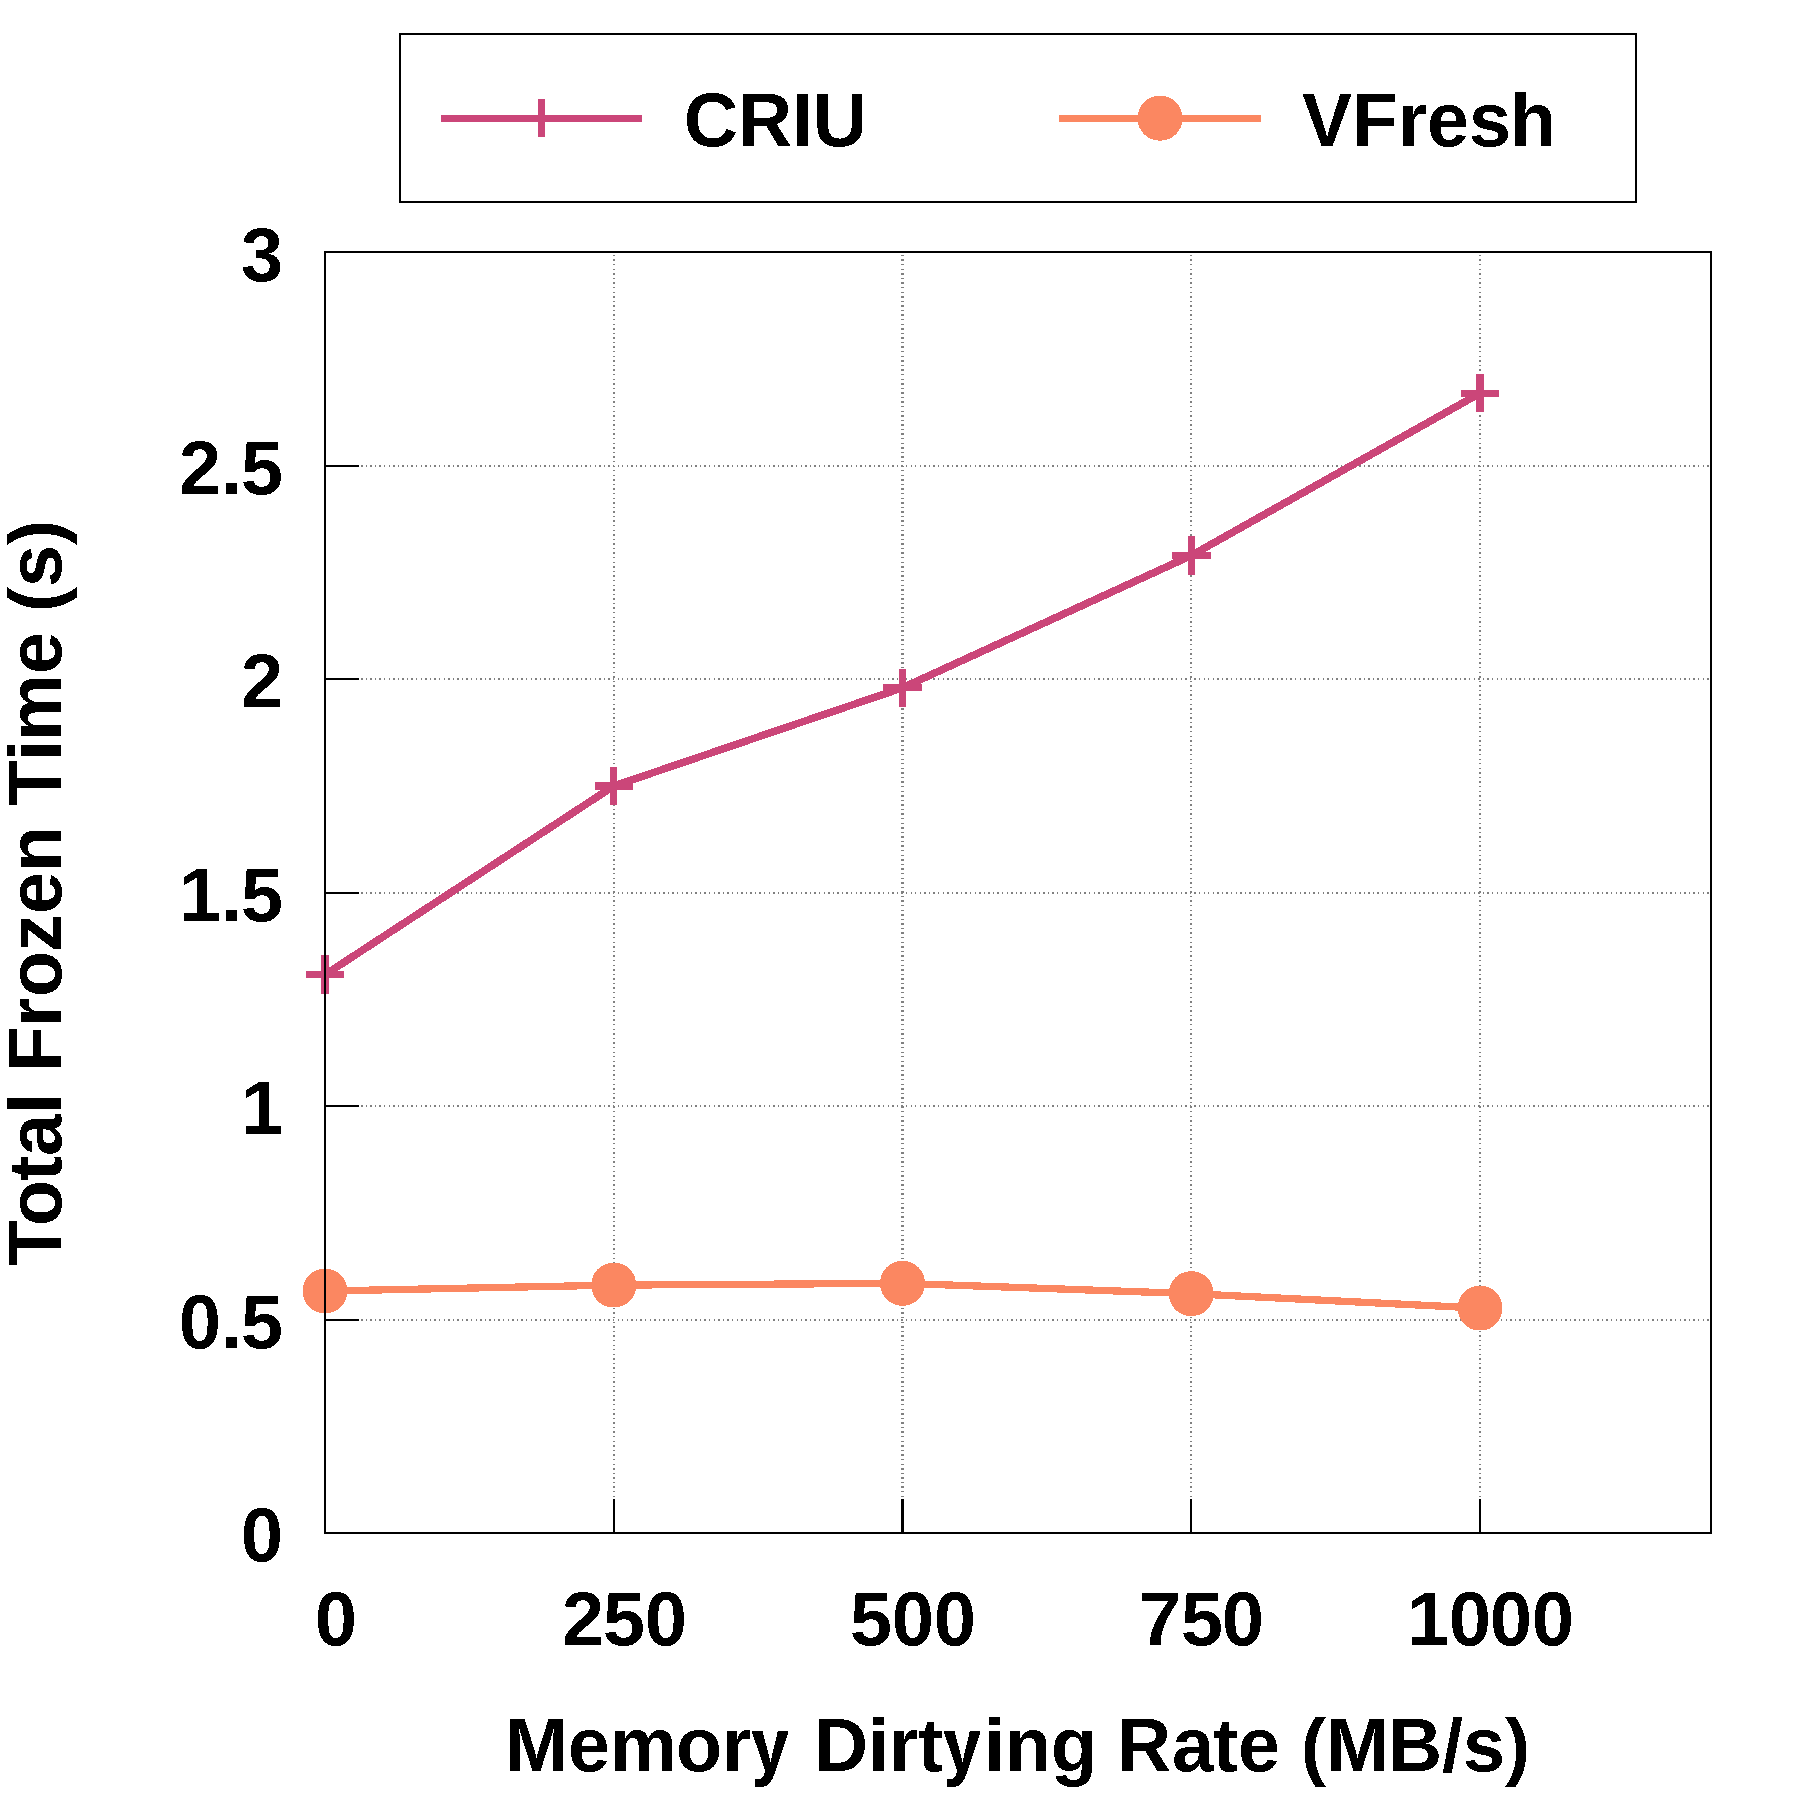
\includegraphics[width=.5\textwidth]{figures/memory_dirty_rate_process_migration_tft.pdf}}
%	\caption{Memory Dirtying Rate Variations}
%	\label{fig:variation1}
%\end{figure*}

%%%%%%%%% DATA for Figure 12 a %%%%%%%%
%		Vfresh	CRIU
%0		0.571	2.56
%250	0.587	5.87
%500	0.591	7.19
%750	0.566	8.58
%1000	0.532	10.23

%%%%%%%%% DATA for Figure 12 b %%%%%%%%
%		Vfresh	CRIU
%0		0.567	1.308
%250	0.581	1.75
%500	0.585	1.98
%750	0.561	2.29
%1000	0.527	2.67

%\begin{figure}
%	\centering
%	
%	\subfloat[Total Migration Time]{
%		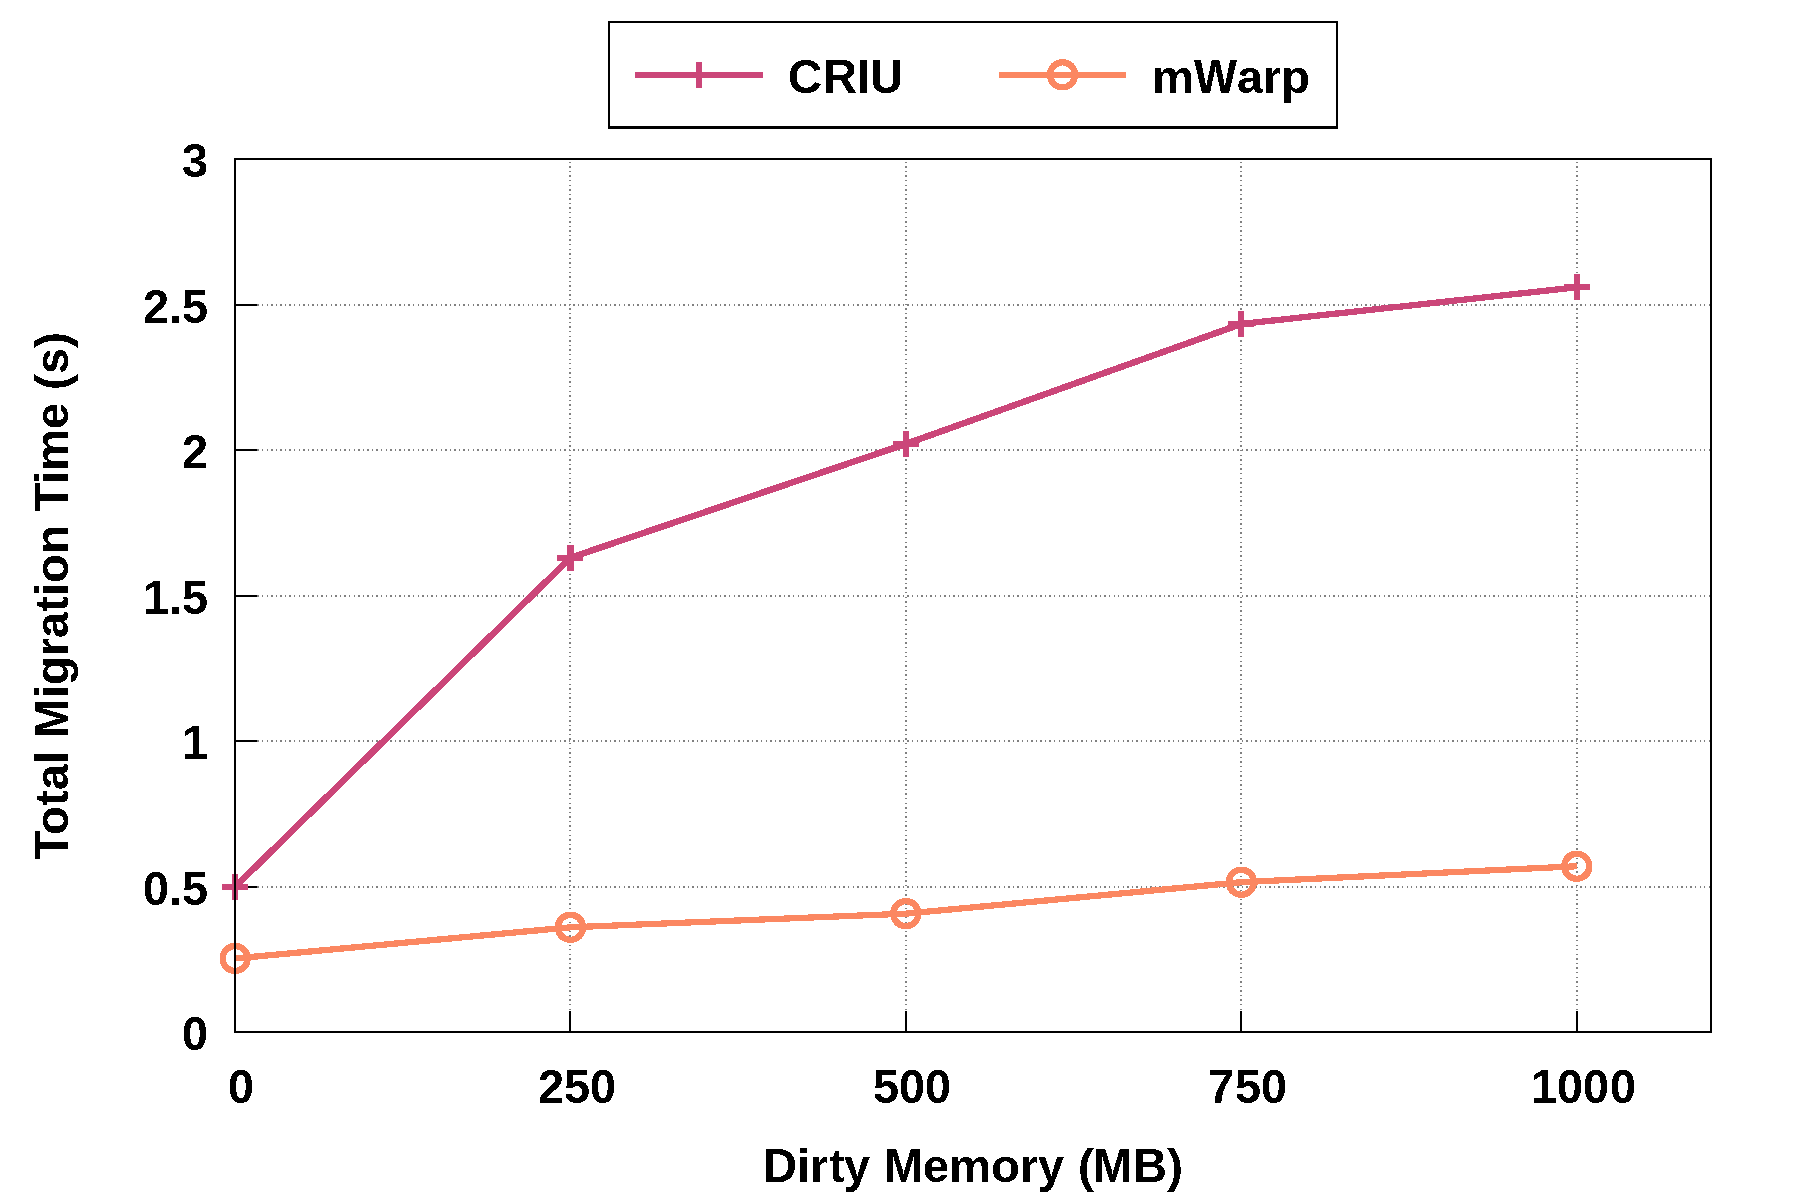
\includegraphics[width=.25\textwidth]{figures/busy_process_migration.pdf}}
%	\subfloat[Total Frozen Time]{
%		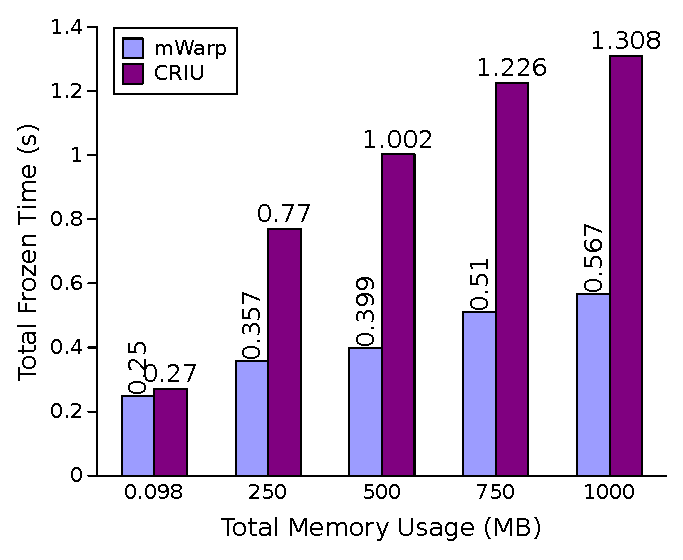
\includegraphics[width=.25\textwidth]{figures/total_mem_usage_TFT.eps}}
%	\caption{Memory Size Variations}
%	\label{fig:variation1}
%\end{figure}
%\begin{figure}
%	\centering
%	
%	\subfloat[Total Migration Time]{
%		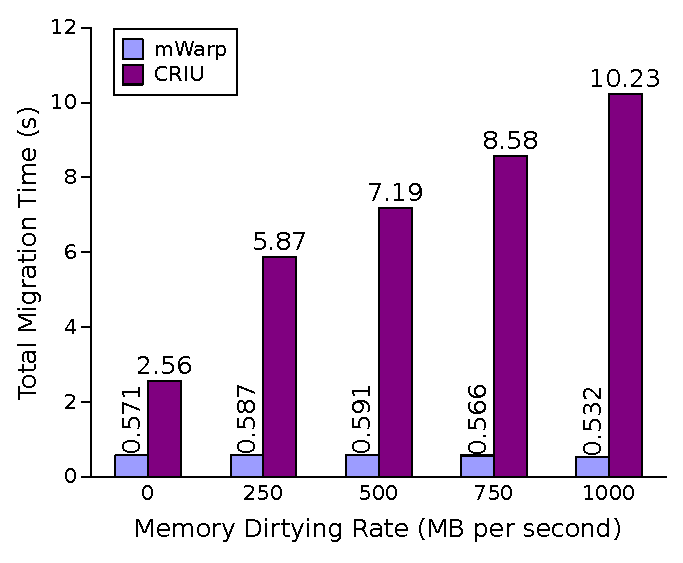
\includegraphics[width=.25\textwidth]{figures/memory_dirtying_TMT.eps}}
%	\subfloat[Total Frozen Time]{
%		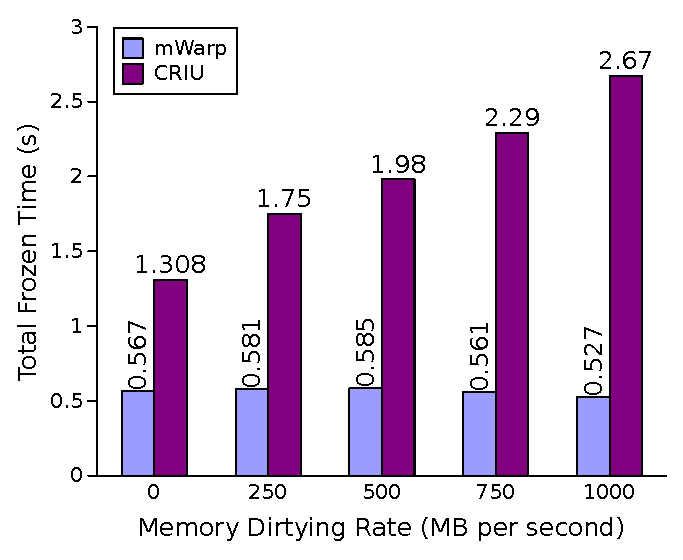
\includegraphics[width=.25\textwidth]{figures/memory_dirtying_TFT.eps}}
%	\caption{Memory Dirtying Rate Variations}
%	\label{fig:variation2}
%\end{figure}

%Figure \ref{fig:variation1} shows the total migration time and the total frozen time of a process that is using varying size of the memory. Our starting point is a process using minimal memory and then we increase the memory usage to see the effect of the total memory size on the total migration time and total frozen time.









%\begin{figure} 
%	\centering
%	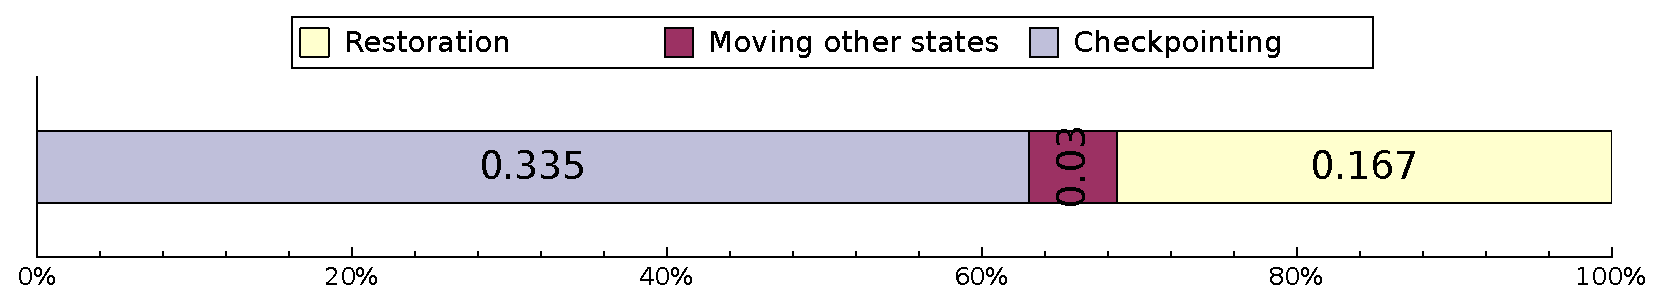
\includegraphics[width=0.5\textwidth]{figures/comapped_bk.eps}
%	\caption{mWarp's Total Frozen Time Breakdown}
%	\label{fig: breakdown2}
%\end{figure}

%We consider the case, where we allocate 1GB and dirties it at 1GB per second continuously, to show the breakdown of the total frozen time during the migration. Figure \ref{fig: breakdown2} show migration causes downtime in the execution of the process during checkpointing, moving the other states and restoration. 


%\begin{figure*}
%	\centering
%	\subfloat[Frozen time breakdown during checkpointing.]{
%		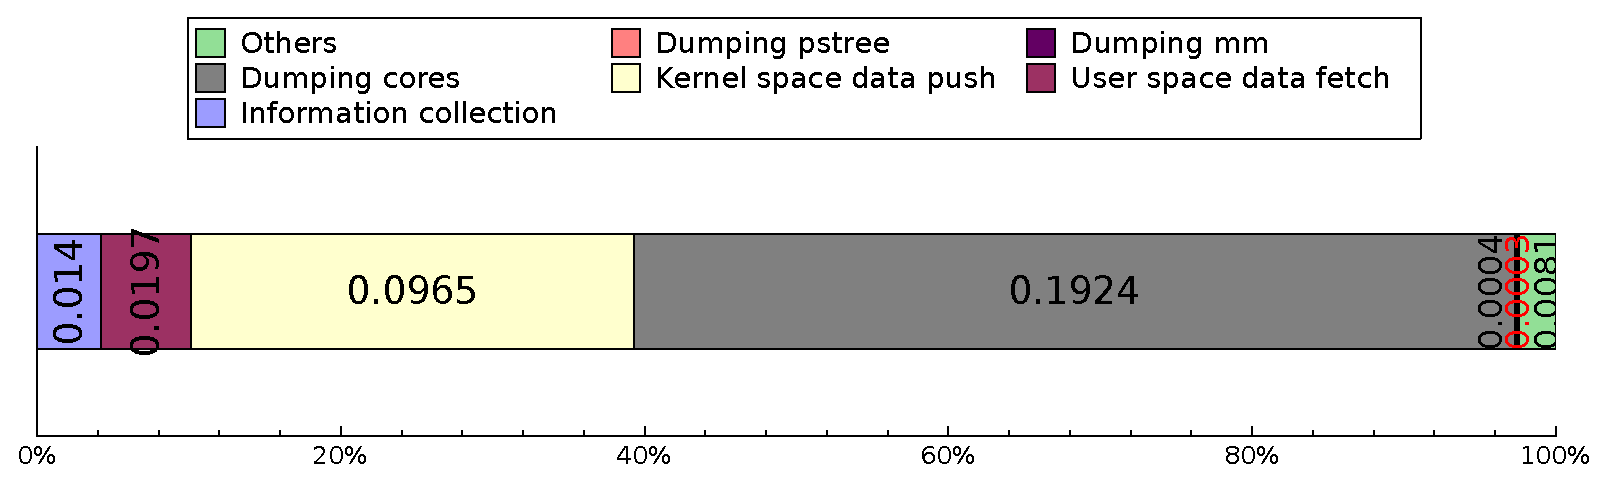
\includegraphics[width=.5\textwidth]{figures/comapped_chkpnt_bk.eps}}
%		\hspace{0.1in}
%	\subfloat[Frozen time breakdown during restoration.]{
%		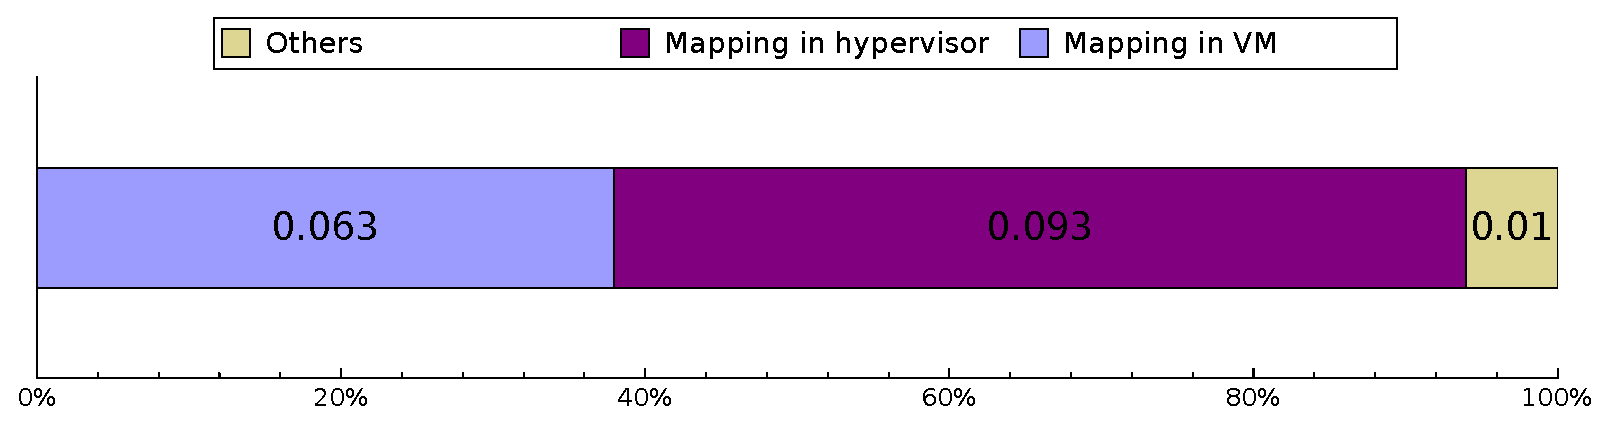
\includegraphics[width=.450\textwidth]{figures/comapped_rst_bk.eps}}
%		%\hspace{0.1in}
%		\vspace{-0.1in}
%	\caption{mWarp's Frozen Time Breakdown During Migration Stages}
%	\vspace{-0.2in}
%	\label{fig: breakdown3}
%\end{figure*}

%Figure \ref{fig: breakdown3} shows the further breakdown of the frozen time during the checkpointing and restoration stage.
%\begin{figure} 
%	\centering
%	\includegraphics[width=0.45\textwidth]{Figures/quicksort_per_sec.eps}
%	\caption{Quicksort Rate}
%	\label{fig: quicksort}
%\end{figure}

%\begin{figure} 
%	\centering
%	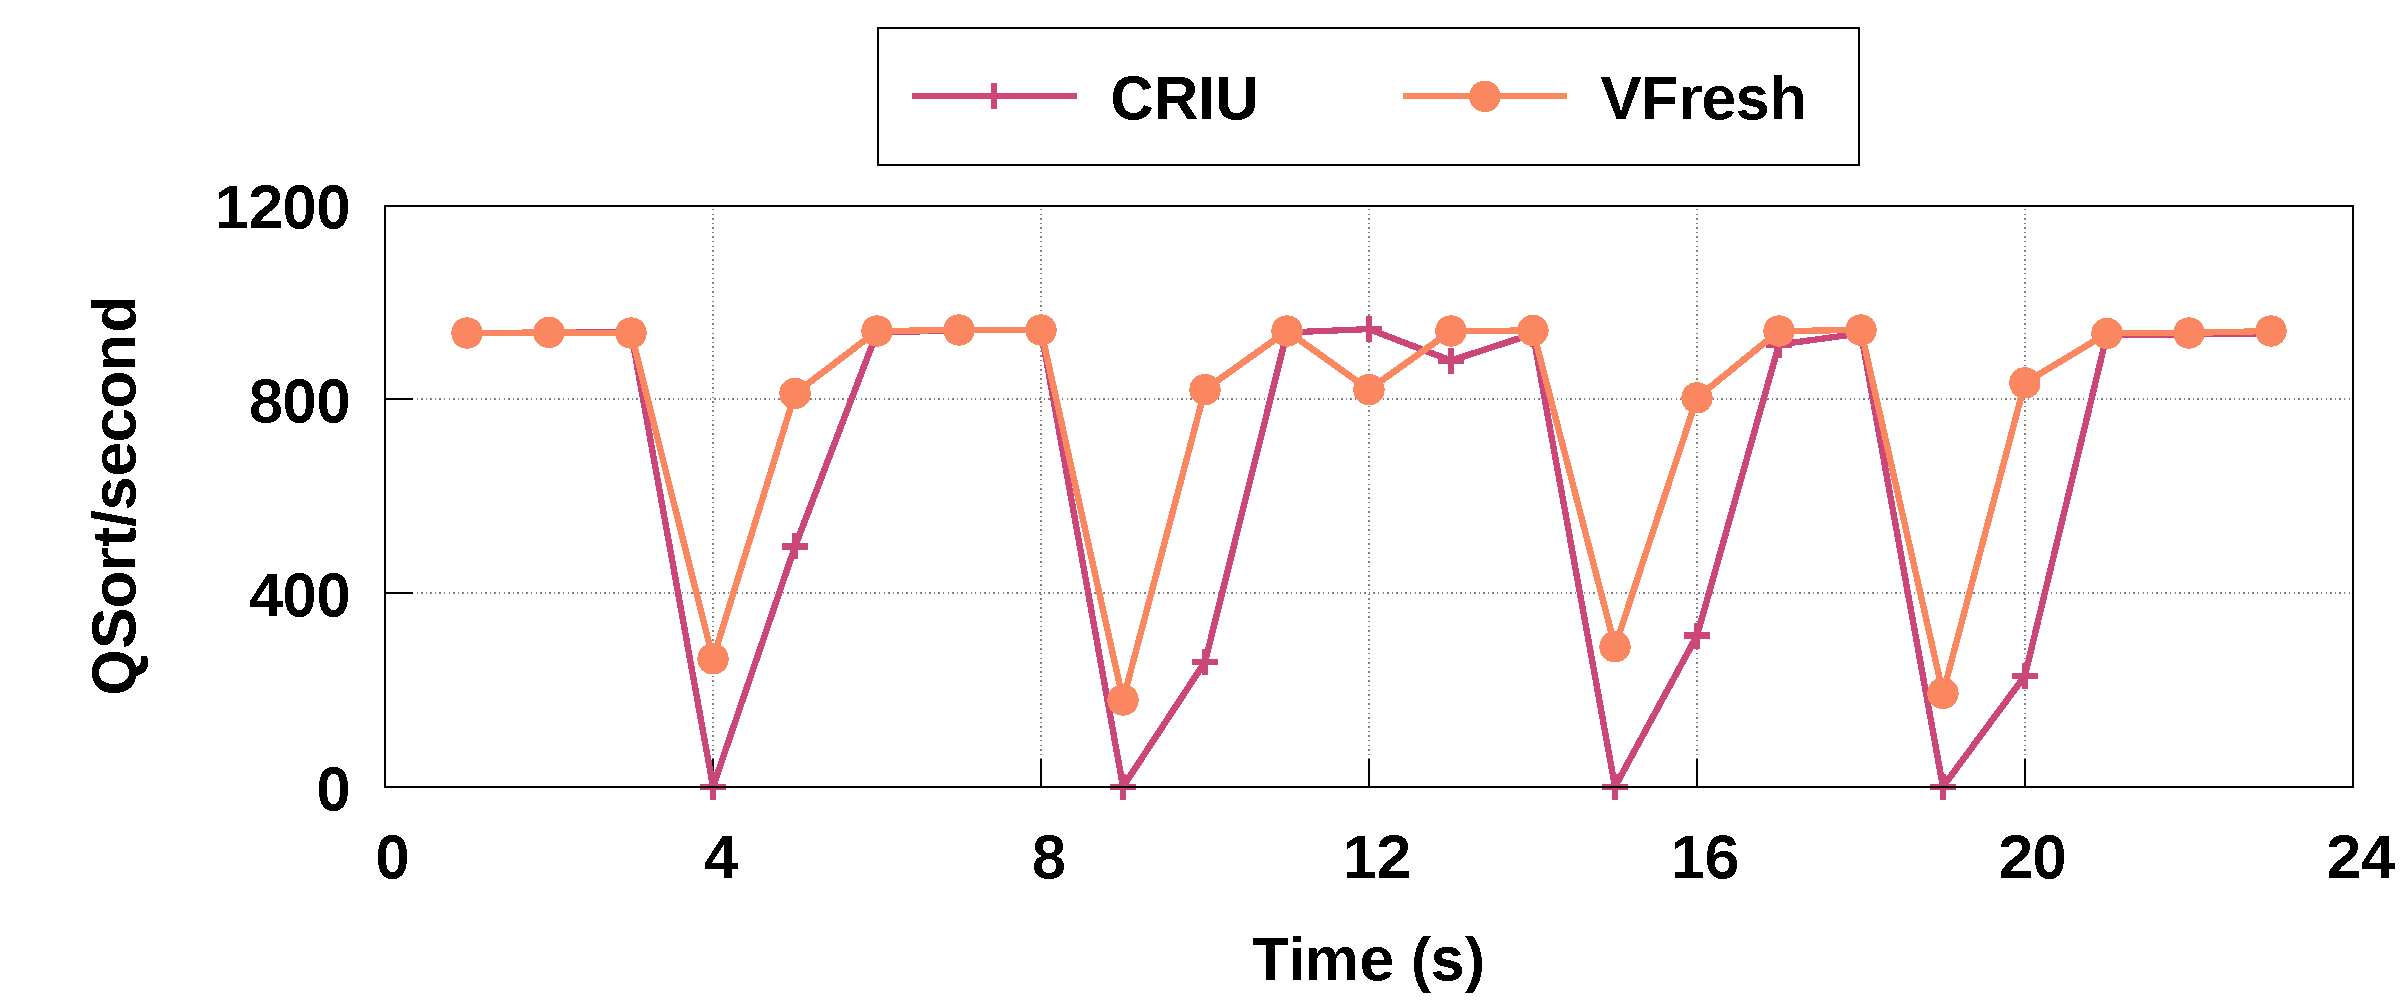
\includegraphics[width=0.5\textwidth]{figures/quicksort_performance.pdf}
%	\caption{Quicksort's Performance}
%	\label{fig: quicksort1}
%\end{figure}

%%%%%%%%% DATA for Figure 13 a %%%%%%%%
%		Baseline VFresh	CRIU
%128	10.014	10.0992	10.6237
%256	10.0366	10.283	11.1255
%512	10.0514	10.4231	11.375
%1024	10.1504	10.4893	12.6827
%%%%%%%%% DATA for Figure 13 b %%%%%%%%
%		VFresh	CRIU
%CN		0.912	2.09
%BS		0.458	1.194
%FQ		0.474	0.86
%FA		0.601	1.561
%SP		0.325	0.626
%BT		0.296	0.575



%\begin{figure*}[t!]
% 	  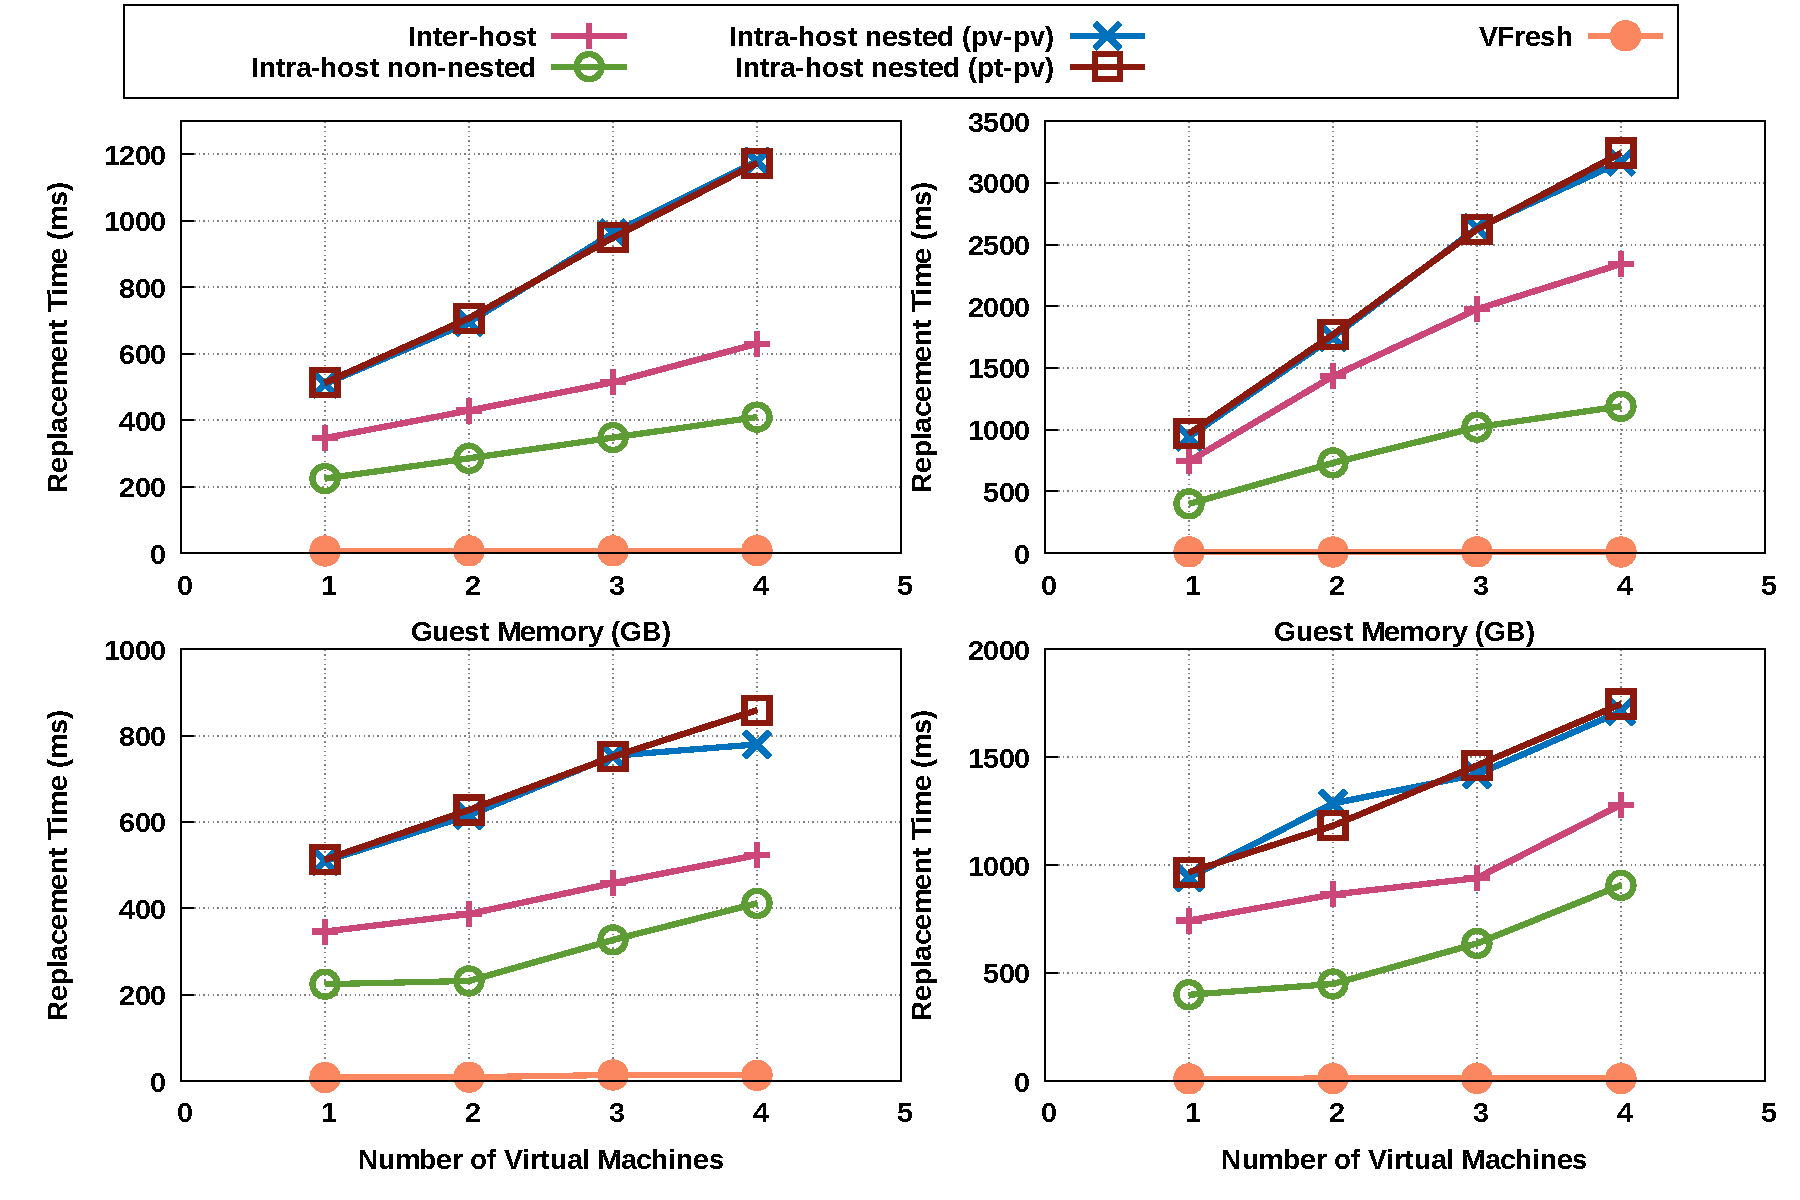
\includegraphics[width=0.98\textwidth]{figures/migration.pdf}
%  \caption{Architecture for hypervisor replacement with direct-device assignment and thin hyperplexor.}
%TODO: Please fix this caption
 % \label{fig:vFresharch}
  %\includegraphics[width=15cm,height=6cm,keepaspectratio]{architecture__1_.jpg}
%\end{figure*}


%\begin{figure} 
%	\centering
%	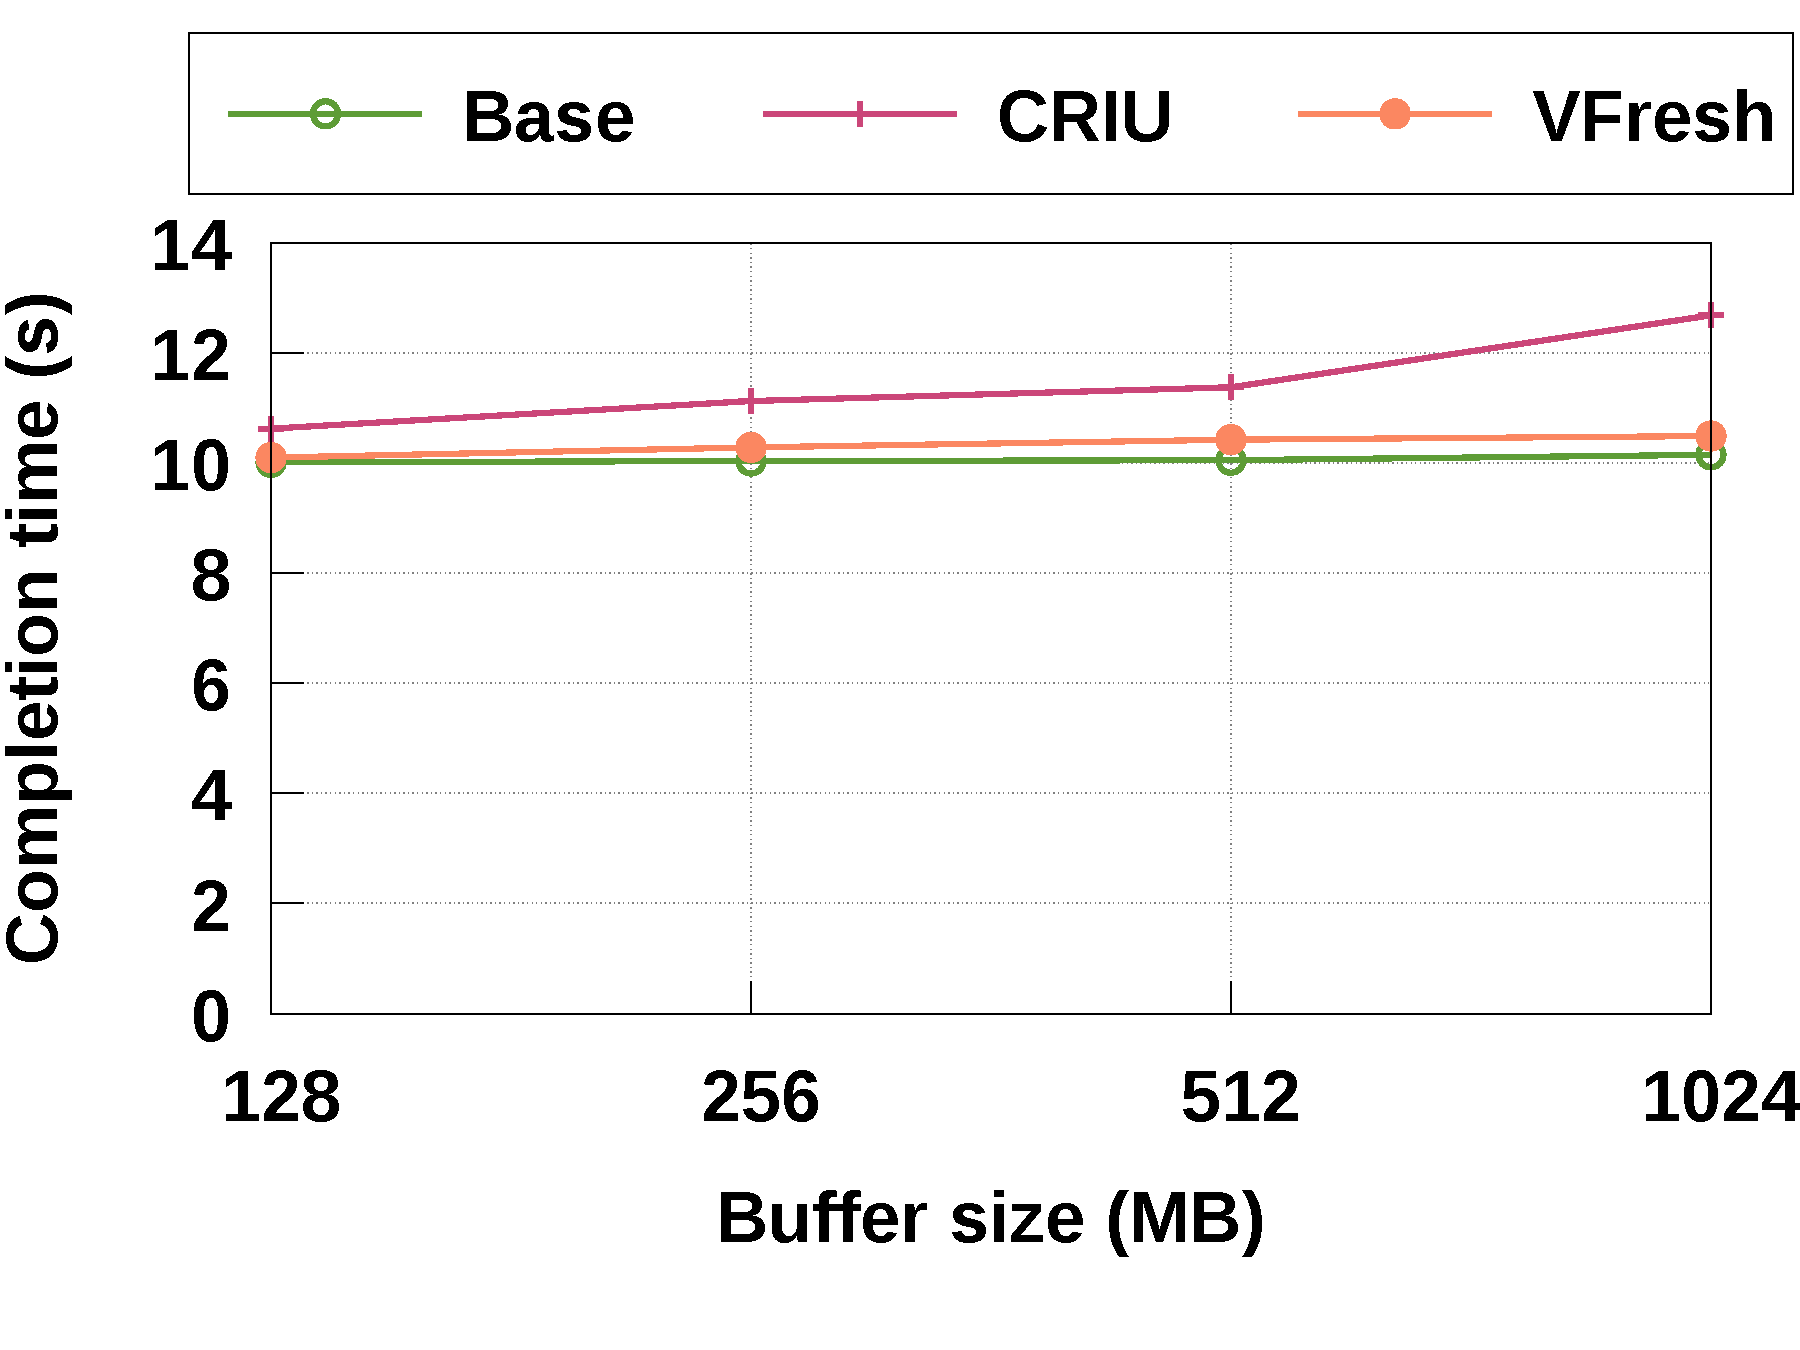
\includegraphics[width=0.5\textwidth]{figures/sysbench_performance.pdf}
%	\caption{Sysbench Performance}
%	\label{fig: sysbench}
%\end{figure}

%\begin{figure} 
%	\centering
%	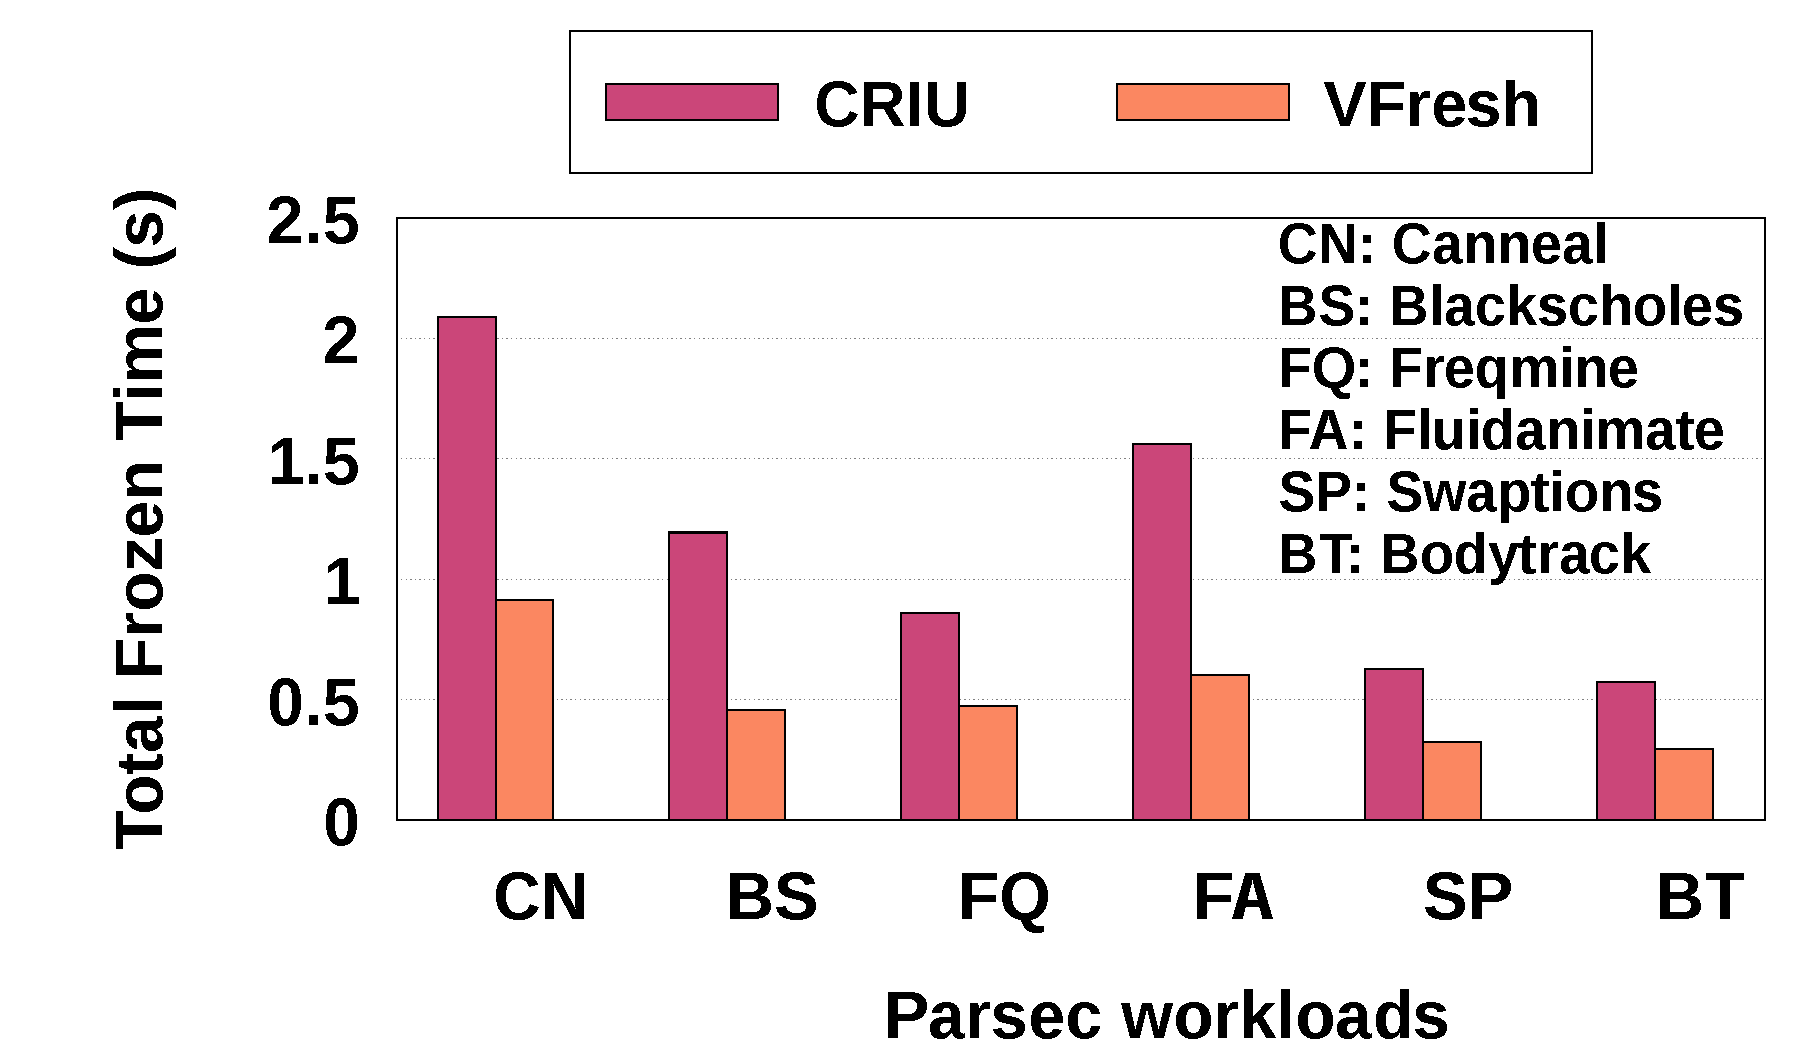
\includegraphics[width=0.5\textwidth]{figures/parsec.pdf}
%	\caption{Downtime Of Parsec Workloads}
%	\label{fig: parsec}
%\end{figure}


